%\section{História da linguagem}

No começo da decada de 90 um pequeno grupo de engenheros da Oracle chamados de ''Green Team'' acreditava que a próxima onde de na area da computação seria a união de equipamentos eletroeletrônicos com os computadores. O ''Green Team'' liderado por James Gosling, demonstraram que a linguagem de programaçao Java, que foi desenvolvida pela equipe e originalmente era chamado de Oak, foi desenvolvida para dispositivos de entretenimento como aparelhos de tv a cabo, porem não foi bem aceita no meio. Em 1995 com a massificação da Internet, a linguagem Java teve sua primeira grande aplicação o navegador Netscape.

Java é uma linguagem de programação de propósito geral orientada a objetos, concebida especificadademente para ter poucas dependencias de implementação que isso acarreta que uma vez que a aplicação fora desenvolvida ela poderá ser executada em qualquer ambiente computacional.

Na sua primeira versão chamada de Java 1 (\acs{JDK} 1.0.2) haviam oito pacotes básicos do java como: java.lang, java.io, java.util, java.net, java.awt, java.awt.image, java.awt.peer e java.applet. Foi usado para o desenvolvimento de ferramentas populares na epoca como o Netscape 3.0 e o Internet Explorer 3.0.

Sua segunda versão foi o \acs{JDK}1.1 \cite{JDK1.1} que trouxe ganhos em funcionalidades, desempenho e qualidade. Novas aplicações tambem surgiram como : JavaBeans, aprimoramento do \acs{AWT}, novas funcionalidades como o \acs{JDBC}, acesso remoto ao objeto \acs{RMI} e suporte ao padrão Unicode 2.0.

A terceira versão Java 2 (\acs{JDK} 1.2) ofereceu melhorias significativas no desempenho, um novo modelo de segurança, flexível e um conjunto completo de aplicações de programação interfaces \acs{API}'s. Os novos recursos da plataforma Java 2 incluiram: 
\begin{itemize}
  \item O modelo de "sandbox"  foi ampliado para dar aos desenvolvedores, usuários e administradores de sistema a opção de especificar e gerenciar um conjunto de políticas de segurança flexíveis que governam as ações de uma aplicação ou applet que pode ou não ser executada.
  \item Suporte nativo a thread para o ambiente operacional Solaris. Compressão de memória para classes carregadas. Alocação de memória com mais desempenho e melhor para a coleta de lixo. Arquitetura de máquina virtual conectável para outras máquinas virtuais, incluindo a Java HotSpot VMNew. Just in Time (JIT). Java Native Interface \acs{JNI} de conversão.
  \item O conjunto de componentes de projeto, \acs{GUI} (Swing). \acs{API} Java 2D que fornece novos recursos gráficos 2D e \acs{AWT}, bem como suporte para impressão. O Java {\it look and fell}. Uma nova API de acessibilidade.
  \item Framework de entrada de caracteres (suporte a japonês, chinês e coreano). Complexo de saída usando a \acs{API} do Java 2D para fornecer um {\it display} bi-direcional, de alta qualidade de japonês, árabe, hebraico e outras línguas de caracteres.
  \item Java Plug-in para navegadores da web, incluída na plataforma Java 2, fornecendo um tempo de execução totalmente compatível com a máquina virtual Java amplamente implantadas em navegadores.
  \item Invocação das operações ou serviços de rede remoto. Totalmente compatível com Java ORB e incluído no tempo de execução.
  \item \acs{JDBC} que fornece um acesso mais fácil aos dados para consultas mais flexíveis. Melhor desempenho e estabilidade são promovidos por cursores de rolagem e suporte para SQL3 de tipos.
\end{itemize}

Em 8 de Maio de 2000 foi anunciado o Java 2 versão 1.3 que trouxe ganho de desempenho em relação a primeira versão da JS2E de cerca de 40\%  no tempo de {\it  start-up}. Tambem trouxe novas funcionaliadades como: 

\begin{itemize}
  \item O Java HotSpot VM de cliente e suas bibliotecas atentando ao desempenho ao fazer o J2SE versão 1.3 a {\it realease} o mais rápido até à data.
  \item Novos recursos, como o {\it caching applet} e instalação do pacote opcional Java através da tecnologia Java {\it  Plug-in} para aumentar a velocidade e a flexibilidade com que os {\it applets} e aplicativos baseados na tecnologia Java pode ser implantado. Java {\it  Plug-in} tecnologia é um componente do ambiente de execução Java 2 que permite Java {\it applets} e aplicativos para a execução.
  \item O novo suporte para \acs{RSA} assinatura eletrônica, gerenciamento de confiança dinâmico, certificados X.509, e verificação de arquivos o que significa o aumento das possibilidades que os desenvolvedores tem para proteger dados eletrônicos.
  \item Uma série de novos recursos e ferramentas de desenvolvimento da tecnologia J2SE versão 1.3 que permite o desenvolvimento mais fácil e rápido de aplicações baseadas na tecnologia {\it web} ou Java {\it  standalone} de alto desempenho.
  \item A adição de RMI/IIOP e o JNDI para a versão 1.3, melhora na interoperabilidade J2SE. RMI/IIOP melhora a conectividade com sistemas de {\it  back-end} que suportam CORBA. JNDI fornece acesso aos diretórios que suportam o populares LDAP Lightweight Directory Access Protocol, entre outros.
\end{itemize}

No ano de 2002 no dia 6 de Fevereiro, foi lançado a J2SE versão 1.4. Com a versão 1.4, as empresas puderam usar a tecnologia Java para desenvolver aplicativos de negócios mais exigentes e com menos esforço e em menos tempo. As novas funcionalidades como a nova I/O e suporte a 64 bits. A J2SE se tornou plataforma ideal para a mineração em grande escala de dados, inteligência de negócios, engenharia e científicos. A versão 1.4 forneceu suporte aprimorado para tecnologias padrões da indústria, tais como SSL, LDAP e CORBA a fim de garantir a operacionalidade em plataformas heterogêneas, sistemas e ambientes. Com o apoio embutido para XML, a autenticação avançada, e um conjunto completo de serviços de segurança, está versão forneceu base para padrões de aplicações Web e serviços interoperáveis. O J2SE avançou o desenvolvimento de aplicativos de cliente com novos controles de GUI, acelerou Java 2D, a performance gráfica, internacionalização e localização expandida de apoio, novas opções de implantação e suporte expandido para o até então Windows XP.\\

Com a chegada da \acs{JSE2} versão 1.5 (Java 5.0) em 30 de Setembro de 2004, impulsionou benefícios extensivos para desenvolvedores, incluindo a facilidade de uso, desempenho global e escalabilidade, monitoramento do sistema e gestão e desenvolvimento. O Java 5 foi derivado do trabalho de 15 componentes Java Specification Requests (JSRs) englobando recursos avançados para a linguagem e plataforma. Os líderes da indústria na época que participam no grupo de peritos J2SE 5.0 incluiram: Apache Software Foundation, Apple Computer, BEA Systems, Borland Software Corporation, Cisco Systems, Fujitsu Limited, HP, IBM, Macromedia, Nokia Corporation, Oracle, SAP AG, SAS Institute, SavaJe Technologies e Sun Microsystems.

Novas funcionalidades foram implementadas como:

\begin{itemize}
  \item Facilidade de desenvolvimento: os programadores da linguagem Java pode ser mais eficiente e produtivos com os recursos de linguagem Java 5 que permitiram a codificação mais segura. Nesta versão surgiu o {\it Generics} ~\cite{OracleGenerics, bracha1998gj}, tipos enumerados, metadados e autoboxing de tipos primitivos permitindo assim uma fácil e rápida codificação.
  
  \item Monitoramento e gestão: Um foco chave para a nova versão da plataforma, a aplicativos baseados na tecnologia Java {\it Virtual Machine} que passou a ser monitorado e gerenciado com o {\it built-in} de suporte para Java {\it Management Extensions}. Isso ajudou a garantir que seus funcionários, sistemas de parceiros do cliente permanecessem em funcionamento por mais tempo. Suporte para sistemas de gestão empresarial baseados em SNMP também é viável.
  
  \item Um olhar novo aplicativo, mais moderna, baseada na tecnologia Java padrão e proporciona uma sensação GUI para aplicativos baseados na tecnologia Java. A J2SE 5.0 teve suporte completo a internacionalização e também possuindo suporte para aceleração de hardware por meio da API OpenGL e tambem para o sistema operacional Solaris e sistemas operacionais da distribuição Linux.
  
  \item Maior desempenho e escalabilidade: A nova versão incluiu melhorias de desempenho, tais como menor tempo de inicialização, um menor consumo de memória e JVM auto ajustável para gerar maior desempenho geral do aplicativo e desenvolvimento em J2SE 5.0 em relação às versões anteriores.
\end{itemize}

Java 1.6 (Java 6) foi divulgado em 11 de dezembro de 2006. Tornou o desenvolvimento mais fácil, mais rápido e mais eficiente em termos de custos e ofereceu funcionalidades para serviços web, suporte linguagem dinâmica, diagnósticos e aplicações desktop. Com a chegada dessa nova versão do Java houve combinação com o NetBeans IDE 5.5 fornecendo aos desenvolvedores uma estrutura confiável, de codigo aberto e compatível, de alta performance para entregar aplicativos baseados na tecnologia Java mais rápido e mais fácil do que nunca. O NetBeans IDE fornece uma fonte aberta e de alto desempenho, modular, extensível, multi-plataforma Java IDE para acelerar o desenvolvimento de aplicações baseadas em software e serviços {\it web}.
Novas funcionalidades foram implementadas como:

\begin{itemize}
  \item O Java 1.6 ajudou a acelerar a inovação para o desenvolvedor, aplicativos de colaboração {\it online} e baseadas na {\it web}, incluindo um novo quadro de desenvolvedores \acs{API}'s para permitir a mistura da tecnologia Java com linguagens de tipagem dinâmica, tais como PHP, Python, Ruby e tecnologia JavaScript. A Sun também criou uma coleção de mecanismos de script e pré-configurado o motor JavaScript Rhino na plataforma Java. Além disso, o software inclui uma pilha completa de clientes de serviços web e suporta as mais recentes especificações de serviços {\it web}, como \acs{JAX-WS} 2.0, \acs{JAXB} 2.0, \acs{STAX} e \acs{JAXP}.
  \item A plataforma Java 1.6 forneceu ferramentas expandidas para o diagnóstico, gestão e monitoramento de aplicações e também inclui suporte para o novo NetBeans Profiler 5.5 para Solaris DTrace e, uma estrutura de rastreamento dinâmico abrangente que está incluído no sistema operacional Solaris 10. Além disso, o software Java SE 6 aumenta ainda mais a facilidade de desenvolvimento com atualizações de interface ferramenta para o Java Virtual Machine (\acs{JVM}) e o Java Platform Debugger Architecture (\acs{ACDP}).
\end{itemize}

Java 7 ~\cite{JSE7} foi lançado no dia 28 de julho de 2011. Essa versão foi resultado do desenvolvimento de toda a indústria envolvendo uma revisão de codigo aberto e extensa colaboração entre os engenheiros da {\it Oracle} e membros do ecossistema Java em todo o mundo através da comunidade {\it OpenJDK} e do {\it Java Community Process} (\acs{JCP}). Compatibilidade com versões anteriores de Java 7 com versões anteriores da plataforma a fim de preservar os conjuntos de habilidades dos desenvolvedores de software Java e proteger os investimentos em tecnologia Java.

Com essa versão novas funcionalidades foram adicionadas:

\begin{itemize}
  \item As alterações de linguagem ajudaram a aumentar a produtividade do desenvolvedor e simplificar tarefas comuns de programação, reduzindo a quantidade de código necessário, esclarecendo sintaxe e tornar o código com mais legibilidade.
  \item Melhor suporte para linguagens dinâmicas incluindo: Ruby, Python e JavaScript, resultando em aumentos substanciais de desempenho no \acs{JVM}.
  \item Uma nova API {\it multicore-ready} que permite aos desenvolvedores para se decompor mais facilmente problemas em tarefas que podem ser executadas em paralelo em números arbitrários de núcleos de processador.
  \item Uma interface de I/O abrangente para trabalhar com sistemas de arquivos que podem acessar uma ampla gama de atributos de arquivos e oferecem mais informações quando ocorrem erros.
  \item Novos recursos de rede e de segurança. Suporte expandido para a internacionalização, incluindo suporte a Unicode 6.0. Versões atualizadas das bibliotecas padrão.\\
\end{itemize}

Com o lançamento do Java SE 8 em 18 de Março de 2014, permitiu uma maior produtividade e desenvolvimento de aplicativos significativos aumentos de desempenho através da redução de linhas de código, {\it collectons} melhoradas, modelos mais simples de programação paralela e uso mais eficiente de processadores multi-core modernos.As principais características do \acs{JDK} 8 são o Projeto Lambda, Nashorn JavaScript Engine, um conjunto de perfis compactas e a remoção da "geração permanente" do HotSpot Java Virtual Machine (\acs{JVM}). A \acs{JDK} 8 alcançou desempenho recorde mundial para 4 sistemas de soquete em servidores baseados em Intel e NEC por 2 sistemas de soquete em servidores SPARC da Oracle T5, com uma melhoria de desempenho de 12\% para 41\% em comparação com o JDK 7 na mesma configuração de Oracle.
O \acs{JDK} 8 adicionou novas funcionalidades como:
  \begin{itemize}
  \item As expressões lambda são suportados pelas seguintes características: As referências a metodos são compactas, maior legibilidade expressões lambda para métodos que já têm um nome. Métodos padrão que permitem adicionar novas funcionalidades para as interfaces de suas bibliotecas e assegurar a compatibilidade binária com o código escrito para versões mais antigas dessas interfaces. Eles são os métodos de interface que têm uma aplicação e a palavra-chave padrão no início da assinatura do método. Além disso, pode-se definir métodos estáticos em interfaces. Novos e aprimorados APIs que se aproveitam de expressões lambda e dos {\it streams} em Java 8 descrevem as classes novos e aprimorados que se aproveitam de expressões lambda e {\it streams}.
  \item O compilador Java aproveita digitação alvo para inferir os parâmetros de tipo de um método de invocação genérica. O tipo de destino de uma expressão é o tipo de dados que o compilador Java espera, dependendo de onde a expressão aparece. Por exemplo, você pode usar o tipo de destino de uma instrução de atribuição para o tipo de inferência em Java 7. No entanto, em Java 8, você pode usar o tipo de destino para a inferência de tipos em mais contextos.
  \item Anotações sobre tipos Java. Agora é possível aplicar uma anotação em qualquer lugar onde um tipo é usado. Utilizado em um conjunto com um sistema de tipo de conector, isso permite a verificação de tipo mais forte de seu código.
  \item  Repetindo Anotações. Agora é possível aplicar o mesmo tipo de anotação mais de uma vez para a mesma declaração ou o tipo de utilização.
  \end{itemize}


								
%\chapter{Fundamentação}
\section {Aspectos evolutivos da liguagem Java}
		\subsection {Java 2}
			A primeira versão do Java Security, disponível no \acs{JDK} 1.1 \cite{JDK1.1}, contém um subconjunto dessa funcionalidade, incluindo \acs{API}'s para:
		  \begin{itemize}
			  \item Assinaturas Digitais: Algoritmos de assinatura digital, como \acs{DSA} ou \acs{MD5} com \acs{RSA}. A funcionalidade inclui a geração de chaves público/privado , bem como assinatura e verificação de dados digitais.
			  \item Gerenciamento de Chaves: Um conjunto de abstrações para o gerenciamento de ''diretores'' (entidades como usuários individuais ou grupos), suas chaves, e os seus certificados. Ele permite que aplicativos para projetar seu próprio sistema de gerenciamento de chaves, e para interoperar com outros sistemas em alto nível.
			  \item Lista de controle de acesso: Um conjunto de abstrações para o gerenciamento de ''diretores'' e suas permissões de acesso.
			  \item A obtenção de um objeto de assinatura: 
			  
\begin{lstlisting}
import java.security.Signature;
import java.security.NoSuchAlgorithmException;
	
public class SignFile {
	Signature signature;
		
	private void init(String algorithm) throws NoSuchAlgorithmException{
		signature = Signature.getSignature(algorithm);
    }
}
\end{lstlisting}
			  
			  \item Em versões anteriores, Java suportava apenas {\it top-level} classes, que devem ser membros de pacotes. Na versão 1.1, o programador Java pode agora definir classes internas como membros de outras classes ~\cite{bracha1998gj}, localmente dentro de um bloco de instruções, ou (anonimamente) dentro de uma expressão.
		  
\begin{lstlisting}
public class FixedStack {
	...
	 public java.util.Enumeration elements() {
	     return new FixedStack$Enumerator(this);
	 }
}
		
class FixedStack$Enumerator implements java.util.Enumeration {
	private FixedStack this$0;
	
	FixedStack$Enumerator(FixedStack this$0) {
		this.this$0 = this$0;
		this.count = this$0.top;
	 }
			
	int count;
	public boolean hasMoreElements() {
		return count > 0;
	}
		
	public Object nextElement() {
		if (count == 0)
			throw new NoSuchElementException("FixedStack");
		
		return this$0.array[--count];
	}
}
\end{lstlisting}
			
			\clearpage
			\item Para escrever um objeto remoto \acs{RMI}, escreve-se uma classe que implementa uma ou mais interfaces remotas. 
			
\begin{lstlisting}
package examples.hello;
public interface Hello extends java.rmi.Remote {
	String sayHello() throws java.rmi.RemoteException;
}
\end{lstlisting}
	 
\item HelloImpl.java
\begin{lstlisting}
package examples.hello;

import java.rmi.;
import java.rmi.server.UnicastRemoteObject;

public class HelloImpl extends UnicastRemoteObject implements Hello{
	private String name;
	
	public HelloImpl(String s) throws RemoteException {
		super();
		name = s;
	}
	
	public String sayHello() throws RemoteException {
		return  "Hello World!";
	}
	
	public static void main(String args[]){
	
		System.setSecurityManager(new RMISecurityManager());
	
		try {
			HelloImpl obj = new HelloImpl("HelloServer");
			Naming.rebind("//myhost/HelloServer", obj);
			System.out.println("HelloServer bound in registry");
		} catch (Exception e) {
			System.out.println("HelloImpl err: " + e.getMessage());
			e.printStackTrace();
		}
	}
}
\end{lstlisting}
		\end{itemize}


	\clearpage
	\subsection {Java 4}
	  \begin{itemize}
		  \item {\it Assertion Facility} \cite{JSE8_Enhancements}. As {\it assertions} são expressões booleanas que o programador acredita ser verdade sobre o estado de um programa de computador. Por exemplo, depois de ordenar uma lista o programador pode afirmar que a lista está em ordem crescente. Avaliando as afirmações em tempo de execução para confirmar a sua validade é uma das ferramentas mais poderosas para melhorar a qualidade do código, uma vez que rapidamente se descobre equívocos do programador sobre o comportamento de um programa.
	  \end{itemize}
	
	\subsection {Java 5}
	  \begin{itemize}
		  \item {\it Generics} \cite{JSE8_Enhancements, OracleGenerics, Parnin:ACM2011}. Este novo recurso para o sistema de tipo permite que um tipo ou método operar em objetos de vários tipos, proporcionando em tempo de compilação tipo de segurança. Acrescenta em tempo de compilação um tipo de segurança para as {\it collections} e elimina o trabalho penoso de {\it casting}. Um exemplo do uso de {\it collections} e {\it generics} respectivamente:
\begin{lstlisting}
static void expurgate(Collection c) {
	for (Iterator i = c.iterator(); i.hasNext(); )
		if (((String) i.next()).length() == 4)
			i.remove();
	}
	
static void expurgate(Collection<String> c) {
	for (Iterator<String> i = c.iterator(); i.hasNext(); )
		if (i.next().length() == 4)
			i.remove();
}
\end{lstlisting}
		  
		\item {\it For-Each Loop}. Esta nova estrutura de linguagem elimina o trabalho e erro de propensão de iteradores e variáveis de índice quando a iteração ocorre sobre coleções e arrays. Como a construção evoluiu com o advento dessa nova estrutura:
	
\begin{lstlisting}
void cancelAll(Collection<TimerTask> c) {
	for (Iterator<TimerTask> i = c.iterator(); i.hasNext(); )
	   i.next().cancel();
}
	
void cancelAll(Collection<TimerTask> c) {
	for (TimerTask t : c)
		t.cancel();
}
\end{lstlisting}
	  
	  \clearpage
	  \item {\it Varargs}. Esta nova estrutura tende a eliminar a necessidade de passagem manual de listas de argumentos em um array ao invocar métodos que aceitam de um comprimento variável de uma lista de argumentos. Nas versões anteriores, um método levava um número arbitrário de valores necessários a  criar uma matriz e colocar os valores para a matriz antes de chamar o método.


\begin{lstlisting}
public class Test {
	public static void main(String[] args) {
	  int passed = 0;
	  int failed = 0;
	  for (String className : args) {
	      try {
	          Class c = Class.forName(className);
	          c.getMethod("test").invoke(c.newInstance());
	          passed++;
	      } catch (Exception ex) {
	          System.out.printf("%s failed: %s%n", className, ex);
	          failed++;
	      }
	  }
	  System.out.printf("passed=%d; failed=%d%n", passed, failed);
	}
}
\end{lstlisting}
 
	  \item {\it Autoboxing/Unboxing}. Esta nova estrutura elimina o trabalho de conversão manual entre tipos primitivos (como {\it int}) e os tipos de classes {\it wrapper}
  \end{itemize}
  
  
  
	\subsection {Java 6}
		Não ocorram mudanças ou introdução de novas estruturas na linguagem Java ~\cite{JSE8_Enhancements}.
	
	\subsection {Java 7}
		\begin{itemize}
		  \item {\it Multi Catch} e lançamento de exceções com melhora na verificação de tipos. Um único bloco {\it catch} poderá lidar com mais de um tipo de exceção. Além disso, o compilador executa a análise mais precisa das exceções. Isso permite que o programador especifique tipos de exceção mais específicos na cláusula de uma declaração método. Um exemplo de como era as estruturas que usavam {\it cacths} e com a introdução de {\it multi catch} com o Java 7 ~\cite{JSE7}, respectivamente.
  

\begin{lstlisting}
catch (IOException ex) {
	logger.log(ex);
	throw ex;
}catch (SQLException ex) {
	logger.log(ex);
	throw ex;
}
\end{lstlisting}
\clearpage
\begin{lstlisting}
catch (IOException|SQLException ex) {
	logger.log(ex);
	throw ex;
}
\end{lstlisting}


 \item O {\it try-with-resouces}. A declaração {\it try-with-resouces} é uma instrução {\it try} que declara um ou mais recursos. Um recurso é um objeto que deve ser fechada após o programa terminar com ele. Essa declaração garante que cada recurso é fechada no final da declaração ~\cite{JSE7_Advanced}.
	 
\begin{lstlisting}

public static void writeToFileZipFileContents(
			String zipFileName, String outputFileName) throws java.io.IOException {
	
	java.nio.charset.Charset charset = java.nio.charset.StandardCharsets.US_ASCII;
	java.nio.file.Path outputFilePath = java.nio.file.Paths.get(outputFileName);
	
	try(
		 java.util.zip.ZipFile zf = new java.util.zip.ZipFile(zipFileName);
		 java.io.BufferedWriter writer = java.nio.file.Files.newBufferedWriter(outputFilePath, charset)
	){
	
		for (java.util.Enumeration entries = zf.entries(); entries.hasMoreElements();) {
			 String newLine = System.getProperty("line.separator");
			 String zipEntryName = ((java.util.zip.ZipEntry)entries.nextElement()).getName() + newLine;
			 writer.write(zipEntryName, 0, zipEntryName.length());
		 }
	}
}

\end{lstlisting}
		  
		  \clearpage
		  \item Inferência de tipos para criação de instâncias em {\it generics} \cite{OracleGenerics,bracha1998gj,Parnin:ACM2011}. Com o Java 7 pode-se substituir os argumentos de tipo necessários para invocar o construtor de uma classe genérica com um conjunto vazio de parâmetros de tipo (<>), desde que o compilador infira os argumentos de tipo a partir do contexto. Este par de colchetes angulares é informalmente chamado de diamante.
  
  

\begin{lstlisting}
Map<String, List<String>> myMap = new HashMap<String, List<String>>();
Map<String, List<String>> myMap = new HashMap<>();
	
List<String> list = new ArrayList<>();
list.add("A");

list.addAll(new ArrayList<>());
	
class MyClass<X> {
	<T> MyClass(T t) {
	...
	}
}
\end{lstlisting}
	 
	  \end{itemize}
	  
	  
	\subsection{Java 8}
	  \begin{itemize}
		  \item Melhoria na inferência de tipos. O compilador Java aproveita digitação para inferir os parâmetros de tipo de uma invocação de método genérica. O tipo de destino de uma expressão é o tipo de dados que o compilador Java espera, dependendo de onde a expressão aparece. Por exemplo, pode-se usar o tipo de destino de uma instrução de atribuição para o tipo de inferência em Java 7. No entanto, em Java 8, pode-se usar o tipo de destino para a inferência de tipos em mais contextos. O exemplo mais proeminente está usando tipos de destino de um método de invocação para inferir os tipos de dados dos seus argumentos.

\begin{lstlisting}
	List<String> stringList = new ArrayList<>();
	stringList.add("A");
	stringList.addAll(Arrays.asList());
\end{lstlisting}
		  
		  
		  \item Expressões lambda. Permitem encapsular uma única unidade de comportamento e passá-lo para outro código. Pode-se usar uma expressãos lambda, se quiser uma determinada ação executada em cada elemento de uma {\it collection}, quando o processo for concluído, ou quando um processo encontra um erro. \cite{JSE7} \\
	  \end{itemize}

\clearpage
\begin{lstlisting}
public class Calculator {
	
	interface IntegerMath {
		int operation(int a, int b);   
	}

	public int operateBinary(int a, int b, IntegerMath op) {
		return op.operation(a, b);
	}

	public static void main(String... args) {

		Calculator myApp = new Calculator();
		IntegerMath addition = (a, b) -> a + b;
		IntegerMath subtraction = (a, b) -> a - b;
		System.out.println("40 + 2 = " + myApp.operateBinary(40, 2, addition));
		System.out.println("20 - 10 = " + myApp.operateBinary(20, 10, subtraction));    
		
	}
}
\end{lstlisting}
\chapter{Fundamentaç\~{a}o}

Conforme mencionado no cap\'{i}tulo anterior, 
o principal objetivo deste trabalho de conclus\~{a}o de curso \'{e} 
identificar oportunidades de evoluç\~{a}o de c\'{o}digo 
em projetos que utilizam recursos anteriores aos dispon\'{i}veis 
nas vers\~{o}es 7 e 8 da linguagem Java, 
algo necess\'{a}rio para o contexto de 
reestrutura\c c\~{a}o de c\'{o}digo que visa adequar um c\'{o}digo 
existente para usar constru\c c\~{o}es mais atuais 
de uma determinada de linguagem de programa\c c\~{a}o 
(no caso, a linguagem Java). Importante destacar 
que as vers\~{o}es da linguagem Java mencionadas anteriormente
introduziram novos recursos, tais como: 
\texttt{multi-catch}, \texttt{try-with-resource}, \texttt{switch-string} 
e \texttt{lambda expressions}; e que esse tipo de 
evoluç\~{a}o constitui uma nova perspectiva 
de \textit{refactoring}, que se caracteriza 
por uma transforma\c c\~{a}o de c\'{o}digo que 
preserva comportamento e que passa a usar  
novas constru\c c\~{o}es da linguagem de programa\c c\~{a}o 
(conforme defendido por Overbey and Johnson~\cite{Overbey:2009}). 

Para atingir o objetivo do trabalho de conclus\~{a}o de curso, 
foi necess\'{a}rio estudar temas relacionados 
\`{a} evolu\c c\~{a}o da linguagem Java, engenharia de 
linguagens de software (ou no Ingl\^{e}s \emph{Software 
Language Engineering}) e refatoramento de c\'{o}digo 
(\emph{code refactoring}). Para fornecer uma introdu\c c\~{a}o ao leitor, 
esse cap\'{i}tulo apresenta 
uma vis\~{a}o geral sobre esses temas. Note que n\~{a}o foi objetivo
deste trabalho implementar um mecanismo de transforma\c c\~{a}o 
de c\'{o}digo, mas sim construir um suporte ferramental 
efetivo para compreender como os desenvolvedores usam as 
constru\c c\~{o}es existentes na linguagem Java e {\bf identificar 
oportunidades de melhoria de c\'{o}digo}, algo essencial para 
permitir a atualiza\c c\~{a}o de um c\'{o}digo existente 
que usa constru\c c\~{o}es ultrapassadas de uma 
linguagem de programa\c c\~{a}o. 
 
\section{Evoluç\~{a}o Linguagem Java}\label{sec:evolucaoJava}



No in\'{i}cio dos anos noventa, um grupo de engenheiros da 
Sun Microsystems, chamados de \textit{Green Team}, acreditava 
que a pr\'{o}xima grande \'{a}rea da computaç\~{a}o 
seria a uni\~{a}o de equipamentos eletroeletrônicos com os 
computadores~\cite{}. O \textit{Green Team}, liderado por James Gosling, 
especificou a linguagem de programaç\~{a}o Java, 
inicialmente proposta para dispositivos de entretenimento 
como aparelhos de TV a cabo. Por outro lado, apenas em 1995, 
com a massificaç\~{a}o da Internet, a linguagem Java 
teve sua primeira grande aplicaç\~{a}o: a constru\c c\~{a}o 
de componentes de software para o navegador Netscape.

Java \'{e} uma linguagem de programaç\~{a}o de prop\'{o}sito geral, 
orientada a objetos e concebida para ser independente de plataforma, 
gra\c cas ao uso de uma m\'{a}quina virtual---a 
\emph{Java Virtual Machine} (JVM). Isso permite 
que uma aplica\c c\~{a}o Java
possa ser executada em qualquer ambiente computacional que possui 
uma JVM aderente \`{a} especifica\c c\~{a}o da linguagem.

Na sua primeira vers\~{a}o publicamente dispon\'{i}vel 
(\acs{JDK} 1.0.2), existiam apenas oito bibliotecas 
presentes na especifica\c c\~{a} Java, tais como 
\texttt{java.lang}, \texttt{java.io}, \texttt{java.util},  
\texttt{java.net}, \texttt{java.awt} e \texttt{java.applet}; 
onde as tr\^{e}s \'{u}ltimas favoreciam a constru\c c\~{a}o de 
solu\c c\~{o}es envolvendo mobilidade de c\'{o}digo:
um componente (um applet Java) poderia ser transferido de um 
servidor para um cliente e, dessa forma, 
ser executado em um navegador Web compat\'{i}vel. As caracter\'{i}sticas de 
independ\^{e}ncia de plataforma e a aproxima\c c\~{a}o com a Web fez 
com que a linguagem Java se tornasse bastante popular, passando a ser 
usada em outros dom\'{i}nios (como o desenvolvimento de software 
para cart\~{o}es inteligentes, para jogos eletr\^{o}nicos e para ambientes corporativos) e a ter 
uma evolu\c c\~{a}o natural com a melhoria de desempenho da 
JVM e a incorpora\c c\~{a}o de um conjunto significativo de 
bibliotecas. 

Apesar de toda essa evolu\c c\~{a}o, que 
trouxe uma r\'{a}pida aceita\c c\~{a}o da linguagem, 
mudan\c cas significativas na especifica\c c\~{a}o 
da sem\^{a}ntica da linguagem s\'{o} se 
tornaram publicamente dispon\'{i}veis em 2004, 
com o lan\c camento da vers\~{a}o intitulada 
Java 5.0 (\emph{Java Language Specification 1.5}). As principais 
contribui\c c\~{o}es para a sem\^{a}ntica da linguagem afetavam 
diretamente a produtividade dos desenvolvedores e incluiam 
implementa\c c\~{o}es mais eficientes de bibliotecas 
existentes (como as bibliotecas de IO e as bibliotecas 
para programa\c c\~{a}o concorrente). Relacionadas \`{a} 
perspectiva sem\^{a}ntica, as principais contribui\c c\~{o}es 
da especifica\c c\~{a}o Java 5.0 introduziram o suporte 
a polimorfismo parametrizado (Java Generics) e enumera\c c\~{o}es; 
o uso de constru\c c\~{o}es \texttt{foreach} para iterar 
sobre cole\c c\~{o}es; a possibilidade de defini\c c\~{a}o de m\'{u}ltiplos 
argumentos com a constru\c c\~{a}o \texttt{varargs} (suportados em 
linguagens como C); e o uso do mecanismo intitulado 
\emph{autoboxing} para converter tipos primitivos nas 
classes Java correspondentes. 
As vers\~{o}es da linguagem Java 7 e Java 8 tamb\'{e}m trouxeram, 
em maior ou menor grau de signific\^{a}ncia, extens\~{o}es sint\'{a}ticas 
e sem\^{a}nticas bastante aguardadas pela comunidade de 
desenvolvedores, tais como:

\begin{description}
\item[Java 7] introduziu em 2011 facilidades como (a) suporte ao tipo \texttt{String} 
em senten\c cas condicionais \texttt{switch}, (b) infer\^{e}ncia de tipos 
na instancia\c c\~{a}o de classes gen\'{e}ricas e (c) captura de 
m\'{u}ltiplos tipos de exce\c c\~{a}o. 

\item[Java 8] introduziu em 2014 o suporte a express\~{o}es lambda e a implementa\c c\~{a}o de 
m\'{e}todos \emph{default} em interfaces Java. O suporte a express\~{o}es lambda pode 
ser compreendido como uma evolu\c c\~{a}o da linguagem t\~{a}o significativo 
quanto a introdu\c c\~{a}o de Java Generics, na vers\~{a}o Java 5. Isso porque 
uma s\'{e}rie de novos idiomas (baseadas em \emph{streaming} para programa\c c\~{a}o 
concorrente) est\~{a}o sendo propostos para a linguagem com base em tal constru\c c\~{a}o.   
\end{description} 


%% Sua segunda vers\~{a}o foi o \acs{JDK}1.1 \cite{JDK1.1} que trouxe ganhos em 
%% funcionalidades, desempenho e qualidade. Novas aplicaç\~{o}es tamb\'{e}m surgiram como : JavaBeans, aprimoramento do \acs{AWT}, novas funcionalidades como o \acs{JDBC}, acesso remoto ao objeto \acs{RMI} e suporte ao padr\~{a}o Unicode 2.0.

%% A terceira vers\~{a}o Java 2 (\acs{JDK} 1.2) ofereceu melhorias significativas no desempenho, um novo modelo de segurança flex\'{i}vel e um conjunto completo de Interface de Programaç\~{a}o de Aplicaç\~{a}o \acs{API}'s. O modelo de "\textit{sandbox}" foi ampliado para dar aos desenvolvedores, usu\'{a}rios e administradores de sistema a opç\~{a}o de especificar e gerenciar um conjunto de pol\'{i}ticas de segurança flex\'{i}vel que gerenciam as aç\~{o}es de uma aplicaç\~{a}o ou \textit{applet} que pode ou n\~{a}o ser executada. Foi introduzido o suporte nativo a \textit{thread} para o ambiente operacional Solaris e tamb\'{e}m a compress\~{a}o de mem\'{o}ria para classes carregadas. Alocaç\~{a}o de mem\'{o}ria com melhor desempenho e aprimoramento da coleta de lixo. Arquitetura de m\'{a}quina virtual conect\'{a}vel para outras m\'{a}quinas virtuais, incluindo a \textit{Java HotSpot VMNew}. \textit{Java Native Interface }\acs{JNI} de convers\~{a}o. O novo conjunto de componentes de projeto, \acs{GUI} (\textit{Swing}). \acs{API} Java 2D que fornece novos recursos gr\'{a}ficos 2D e \acs{AWT}, bem como suporte para impress\~{a}o. Java \textit{plug-in} para navegadores, fornecendo um tempo de execuç\~{a}o totalmente compat\'{i}vel com a m\'{a}quina virtual Java amplamente implantadas em navegadores. A inclus\~{a}o do \acs{JDBC} que fornece um acesso mais f\'{a}cil aos dados para consultas mais flex\'{i}veis, suporte ao SQL3 e trouxe melhor desempenho e estabilidade promovidos por cursores de rolagem.


%% Em 8 de Maio de 2000 foi anunciado o Java 2 vers\~{a}o 1.3 que trouxe ganho de desempenho em relaç\~{a}o a primeira vers\~{a}o da JS2E de cerca de 40\%  no tempo de {\it  start-up}. O {\it Java HotSpot VM} cliente e suas bibliotecas atentando ao desempenho ao fazer o J2SE vers\~{a}o 1.3 a {\it release} o mais r\'{a}pido at\'{e} à data. Novos recursos, como o {\it caching applet} e instalaç\~{a}o do pacote opcional Java atrav\'{e}s da tecnologia Java {\it  Plug-in} para aumentar a velocidade e a flexibilidade com que os {\it applets} e aplicativos baseados na tecnologia Java podem ser implantados. Java {\it  Plug-in} tecnologia \'{e} um componente do ambiente de execuç\~{a}o Java 2 que permite Java {\it applets} e aplicativos executarem. O novo suporte para \acs{RSA}, assinatura eletrônica, com um gerenciamento mais confi\'{a}vel e din\^{a}mico, certificados X.509, e verificaç\~{a}o de arquivos o que significa aumento das possibilidades que os desenvolvedores tem para proteger dados eletrônicos. Uma s\'{e}rie de novos recursos e ferramentas de desenvolvimento da tecnologia J2SE vers\~{a}o 1.3 que permite o desenvolvimento mais f\'{a}cil e r\'{a}pido de aplicaç\~{o}es baseadas na tecnologia {\it web} ou Java {\it  standalone} de alto desempenho. A adiç\~{a}o de RMI/IIOP e o JNDI para a vers\~{a}o 1.3, melhora na interoperabilidade J2SE. Melhora da conectividade com sistemas de {\it  back-end} que suportam CORBA. O novo suporte que o JNDI fornece acesso aos diret\'{o}rios que suportam o populares LDAP Lightweight Directory Access Protocol, entre outros.


%% No ano de 2002 no dia 6 de Fevereiro, foi lançado a J2SE vers\~{a}o 1.4. Com a vers\~{a}o 1.4, as empresas puderam usar a tecnologia Java para desenvolver aplicativos de neg\'{o}cios mais exigentes e com menos esforço e em menos tempo. As novas funcionalidades como a nova I/O e suporte a 64 bits. A J2SE se tornou plataforma ideal para a mineraç\~{a}o em grande escala de dados, inteligência de neg\'{o}cios, engenharia e cient\'{i}ficos. A vers\~{a}o 1.4 forneceu suporte aprimorado para tecnologias padr\~{o}es da ind\'{u}stria, tais como SSL, LDAP e CORBA a fim de garantir a operacionalidade em plataformas heterogêneas, sistemas e ambientes. Com o apoio embutido para XML, a autenticaç\~{a}o avançada, e um conjunto completo de serviços de segurança, est\'{a} vers\~{a}o forneceu base para padr\~{o}es de aplicaç\~{o}es Web e serviços interoper\'{a}veis. O J2SE avançou para o desenvolvimento de aplicativos de cliente com novos controles de GUI, acelerou Java 2D, a performance gr\'{a}fica, internacionalizaç\~{a}o e localizaç\~{a}o expandida de apoio, novas opç\~{o}es de implantaç\~{a}o e suporte expandido para o at\'{e} ent\~{a}o {\it Windows XP}.

%% Com a chegada da \acs{JSE2} vers\~{a}o 1.5 (Java 5.0) em 30 de Setembro de 2004, impulsionou benef\'{i}cios extensivos para desenvolvedores, incluindo a facilidade de uso, desempenho global e escalabilidade, monitoramento do sistema e gest\~{a}o e desenvolvimento. O Java 5 foi derivado do trabalho de 15 componentes Java Specification Requests (JSRs) englobando recursos avançados para a linguagem e plataforma. Os l\'{i}deres da ind\'{u}stria na \'{e}poca que participam no grupo de peritos J2SE 5.0 incluiram: Apache Software Foundation, Apple Computer, BEA Systems, Borland Software Corporation, Cisco Systems, Fujitsu Limited, HP, IBM, Macromedia, Nokia Corporation, Oracle, SAP AG, SAS Institute, SavaJe Technologies e Sun Microsystems.

%% Houve novas funcionalidades foram implementadas como: facilidade de desenvolvimento onde os programadores da linguagem Java pode ser mais eficiente e produtivos com os recursos de linguagem Java 5 que permitiram a codificaç\~{a}o mais segura. Nesta vers\~{a}o surgiu o {\it Generics} ~\cite{OracleGenerics, bracha1998gj}, tipos enumerados, metadados e autoboxing de tipos primitivos permitindo assim uma f\'{a}cil e r\'{a}pida codificaç\~{a}o. Monitoramento e gest\~{a}o permitindo um foco para a nova vers\~{a}o da plataforma, a aplicativos baseados na tecnologia Java {\it Virtual Machine} que passou a ser monitorado e gerenciado com o {\it built-in} de suporte para Java {\it Management Extensions}. Suporte para sistemas de gest\~{a}o empresarial baseados em SNMP tamb\'{e}m \'{e} vi\'{a}vel. Um olhar novo sobre aplicativos baseado na tecnologia Java padr\~{a}o e proporcionou um melhor desenvolvimento GUI para aplicativos baseados na tecnologia Java. A J2SE 5.0 teve suporte completo a internacionalizaç\~{a}o e tamb\'{e}m inseriu suporte para aceleraç\~{a}o de hardware por meio da {\it API OpenGL } e tamb\'{e}m para o sistema operacional Solaris e sistemas operacionais da distribuiç\~{a}o Linux. **Maior desempenho e escalabilidade com a nova vers\~{a}o que incluiu melhorias de desempenho, reduç\~{a}o no tempo de inicializaç\~{a}o, um menor consumo de mem\'{o}ria e JVM auto ajust\'{a}vel para gerar maior desempenho geral do aplicativo e desenvolvimento em J2SE 5.0 em relaç\~{a}o a vers\~{o}es anteriores.

%% Java 1.6 (Java 6) foi divulgado em 11 de dezembro de 2006. Tornou o desenvolvimento mais f\'{a}cil, r\'{a}pido e eficiente em termos de custos e ofereceu funcionalidades para serviços web, suporte linguagem din\^{a}mica, diagn\'{o}sticos e aplicaç\~{o}es {\it desktop}. Com a chegada dessa nova vers\~{a}o do Java houve combinaç\~{a}o com o {\it NetBeans} IDE 5.5 fornecendo aos desenvolvedores uma estrutura confi\'{a}vel, de c\'{o}digo aberto e compat\'{i}vel, de alta performance para entregar aplicativos baseados na tecnologia Java mais r\'{a}pido e f\'{a}cil do que nunca. O {\it NetBeans} IDE fornece uma fonte aberta e de alto desempenho, modular, extens\'{i}vel, multiplataforma Java IDE para acelerar o desenvolvimento de aplicaç\~{o}es baseadas em software e serviços {\it web}. O Java 1.6 ajudou a acelerar a inovaç\~{a}o para o desenvolvedor, aplicativos de colaboraç\~{a}o {\it online} e baseadas na {\it web}, incluindo um novo quadro de desenvolvedores \acs{API}'s para permitir a mistura da tecnologia Java com linguagens de tipagem din\^{a}mica, tais como PHP, Python, Ruby e tecnologia JavaScript. A Sun tamb\'{e}m criou uma coleç\~{a}o de mecanismos de {\it script} e pr\'{e}-configurado o motor {\it JavaScript Rhino} na plataforma Java. Al\'{e}m disso, o software inclui uma pilha completa de clientes de serviços web e suporta as mais recentes especificaç\~{o}es de serviços {\it web}, como \acs{JAX-WS} 2.0, \acs{JAXB} 2.0, \acs{STAX} e \acs{JAXP}. A plataforma Java 1.6 forneceu ferramentas expandidas para o diagn\'{o}stico, gest\~{a}o e monitoramento de aplicaç\~{o}es e tamb\'{e}m inclui suporte para o novo {\it NetBeans Profiler} 5.5 para {\it Solaris DTrace } e, uma estrutura de rastreamento din\^{a}mico abrangente que est\'{a} inclu\'{i}do no sistema operacional Solaris 10. Al\'{e}m disso, o software Java SE 6 aumenta ainda mais a facilidade de desenvolvimento com atualizaç\~{o}es de interface ferramenta para o {\it Java Virtual Machine} (\acs{JVM}) e o {\it Java Platform Debugger Architecture} (\acs{ACDP}).

%% Java 7 ~\cite{JSE7} foi lançado no dia 28 de julho de 2011. Essa vers\~{a}o foi resultado do desenvolvimento de toda a ind\'{u}stria o que envolveu uma revis\~{a}o de c\'{o}digo aberto e extensa colaboraç\~{a}o entre os engenheiros da {\it Oracle} e membros do ecossistema Java em todo o mundo atrav\'{e}s da comunidade {\it OpenJDK} e do {\it Java Community Process} (\acs{JCP}). Compatibilidade com vers\~{o}es anteriores de Java 7 com vers\~{o}es anteriores da plataforma a fim de preservar os conjuntos de habilidades dos desenvolvedores de software Java e proteger os investimentos em tecnologia Java. As alteraç\~{o}es da linguagem ajudaram a aumentar a produtividade do desenvolvedor e simplificar tarefas comuns de programaç\~{a}o, reduzindo a quantidade de c\'{o}digo necess\'{a}rio, esclarecendo sintaxe e tornar o c\'{o}digo com mais legibilidade. Melhor suporte para linguagens din\^{a}micas incluindo: Ruby, Python e JavaScript, resultando em aumentos substanciais de desempenho no \acs{JVM}. Uma nova API {\it multicore ready} que permite aos desenvolvedores para se decompor mais facilmente problemas em tarefas que podem ser executadas em paralelo em n\'{u}meros arbitr\'{a}rios de n\'{u}cleos de processador. Uma interface de I/O abrangente para trabalhar com sistemas de arquivos que podem acessar uma ampla gama de atributos de arquivos e oferecem mais informaç\~{o}es quando ocorrem erros. Novos recursos de rede e de segurança. Suporte expandido para a internacionalizaç\~{a}o, incluindo suporte a Unicode 6.0. Al\'{e}m de vers\~{o}es atualizadas das bibliotecas padr\~{a}o.

%% Com o lançamento do Java SE 8 em 18 de Março de 2014, permitiu uma maior produtividade e desenvolvimento de aplicativos significativos aumentos de desempenho atrav\'{e}s da reduç\~{a}o de linhas de c\'{o}digo, {\it collectons} melhoradas, modelos mais simples de programaç\~{a}o paralela e uso mais eficiente de processadores {\it multi-core}. As principais caracter\'{i}sticas do \acs{JDK} 8 s\~{a}o o projeto Lambda, {\it Nashorn JavaScript Engine}, um conjunto de perfis compactas e a remoç\~{a}o da "geraç\~{a}o permanente" do {\it HotSpot Java Virtual Machine} (\acs{JVM}). A \acs{JDK} 8 alcançou desempenho recorde mundial para 4 sistemas de soquete em servidores baseados em Intel e NEC por 2 sistemas de soquete em servidores SPARC da Oracle T5, com uma melhoria de desempenho de 12\% para 41\% em comparaç\~{a}o com o JDK 7 na mesma configuraç\~{a}o de Oracle.

%% %O \acs{JDK} 8 adicionou novas funcionalidades como as express\~{o}es lambda com as seguintes caracter\'{i}sticas: referências a m\'{e}todos s\~{a}o compactas e maior legibilidade express\~{o}es lambda para m\'{e}todos que j\'{a} têm um nome. M\'{e}todos padr\~{a}o que permitem adicionar novas funcionalidades para as interfaces de suas bibliotecas e assegurar a compatibilidade bin\'{a}ria com o c\'{o}digo escrito para vers\~{o}es mais antigas dessas interfaces. Eles m\'{e}todos de interface que têm uma aplicaç\~{a}o e a palavra-chave padr\~{a}o no in\'{i}cio da assinatura do m\'{e}todo. Al\'{e}m disso, pode-se definir m\'{e}todos est\'{a}ticos em interfaces. Novos e aprimorados APIs que se aproveitam de express\~{o}es lambda e dos {\it streams} em Java 8 descrevem as classes novos e aprimorados que se aproveitam de express\~{o}es lambda e {\it streams}. Aprimoramento do compilador Java aproveita digitaç\~{a}o alvo para inferir os par\^{a}metros de tipo de um m\'{e}todo de invocaç\~{a}o gen\'{e}rica. O tipo de destino de uma express\~{a}o \'{e} o tipo de dados que o compilador Java espera, dependendo de onde a express\~{a}o aparece, por exemplo, pode-se usar o tipo de destino de uma instruç\~{a}o de atribuiç\~{a}o para o tipo de inferência em Java 7. No entanto, em Java 8, você pode usar o tipo de destino para a inferência de tipos em mais contextos. Anotaç\~{o}es sobre tipos Java onde \'{e} poss\'{i}vel aplicar uma anotaç\~{a}o em qualquer lugar onde um tipo \'{e} usado, utilizado em um conjunto com um sistema de tipo de conector, isso permite a verificaç\~{a}o de tipo mais forte de seu c\'{o}digo e repetiç\~{a}o de anotaç\~{o}es que agora \'{e} poss\'{i}vel aplicar o mesmo tipo de anotaç\~{a}o mais de uma vez para a mesma declaraç\~{a}o ou o tipo de utilizaç\~{a}o.


\section{Engenharia de Linguagens de Software}\label{sec:softEng}


\begin{flushright}
\emph{
\ldots ou engenharia de software para linguagens de programa\c c\~{a}o 
(no Ingl\^{e}s, Software Language Engineering).}
\end{flushright}

A manipulaç\~{a}o de artefatos escritos em 
uma linguagem de programaç\~{a}o (ou em linguagens de software) 
\'{e} uma tarefa desafiadora, mas que permite o desenvolvimento 
de software aplic\'{a}vel a diferentes cen\'{a}rios, mas que permitem, por exemplo, 
manipular arquivos \texttt{XML}, transformar 
informa\c c\~{o}es e scripts presentes 
em bancos de dados legados, efetuar a tradu\c c\~{a}o de programas 
escritos em uma vers\~{a}o desatualizada de uma linguagem. 

Por envolver diferentes est\'{a}gios, o desenho desse tipo de solu\c c\~{a}o requer, geralmente, 
um estilo arquitetural baseado em um \emph{pipeline},  onde cada est\'{a}gio necess\'{a}rio \`{a}  
 manipulaç\~{a}o de uma linguagem \'{e} implementado como um componente de software. Quando combinados, 
tais componentes proporcionam um programa capaz de realizar a tarefa desejada para realizar o processamento 
de uma ou mais linguagens. A Figura:~\ref{fig:stagesLanguageApp} exibe uma organiza\c c\~{a}o 
t\'{i}pica de componentes para o processamento de artefatos escritos em uma linguagem de 
programa\c c\~{a}o, onde a cada est\'{a}gio do \emph{pipeline}, um componente 
utiliza os resultados do est\'{a}gio anterior para gerar uma sa\'{i}da para o componente 
que realiza o processamento no est\'{a}gio posterior.  

\begin{figure}[h]
  \center
  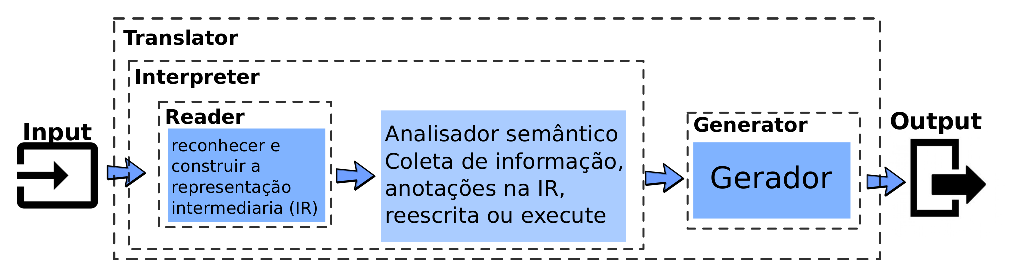
\includegraphics[scale=0.9]{Imagens/stagesLanguageApp}
  \label{fig:stagesLanguageApp}
  \caption{Fases de aplicaç\~{o}es com linguagens.}
\end{figure}

Existe um esforço consider\'{a}vel para tratar a engenharia de linguagens de programaç\~{a}o como sendo o desenvolvimento de um software comum. 
Algumas aplicaç\~{o}es t\'{i}picas deste dom\'{i}nio s\~{a}o \texttt{reconhecedores, interpretadores, tradutores e geradores}, 
conforme menciona Terrance Parr~\cite{Parr:2009:LIP:1823613}. 

%% Um \emph{Reconhecedor} \'{e} uma construç\~{a}o capaz de receber uma estrutura de dado como um input ou um fluxo de inputs. O fluxo de input pode geralmente \'{e} texto puro mas pode ser utilizado dado bin\'{a}rio. Como exemplo de aplicaç\~{a}o tem-se ferramentas analisadoras de referências cruzadas, e ferramentas para carregar classes.

%% \texttt{Interpretador:} Um interpretador, lê uma entrada, decodifica e executa as instruç\~{o}es, interpretadores variam de simples calculadoras at\'{e} a implementaç\~{a}o de linguagens de programaç\~{a}o como Java, Python e PHP.

%% \texttt{Tradutor:}A partir um input de texto ou bin\'{a}rio \'{e} emitido uma sa\'{i}da para uma linguagem que pode ser a mesma ou n\~{a}o. É a combinaç\~{a}o do \textit{reader} e \textit{generator}. Como exemplo tem-se tradutores de linguagens extintas para linguagens atuais, \texttt{refactorers},  gerador de logs e macro pre-processadores.
	
%% \texttt{Gerador:} Percorre uma estrutura de dado e emite uma sa\'{i}da. Como exemplo tem-se ferramentas de mapeamento de objetos relacionais em banco de dados, serializador de objetos, gerador de c\'{o}digo fonte e geradores de p\'{a}gina web.



Al\'{e}m dessas aplica\c c\~{o}es t\'{i}picas, 
ferramentas para a identifica\c c\~{a}o est\'{a}tica de \emph{bugs}, por exemplo, tamb\'{e}m s\~{a}o comumente 
implementadas usando uma organiza\c c\~{a}o como a representada na Figura~\ref{fig:stagesLanguageApp}. 
A ferramenta \textit{FindBugs}~\cite{FindBugs} serve como um exemplo de solu\c c\~{a}o para identifica\c c\~{a}o 
de poss\'{i}veis erros em programas escritos na linguagem Java, a partir do \emph{bytecode} resultante do 
processo de compila\c c\~{a}o. Note na Figura:~\ref{fig:findBugs} a semelhan\c ca arquitetural com as 
abordagens t\'{i}picas para o processamento de artefatos de linguagens de programa\c c\~{a}o. 

\begin{figure}[h]
	\center
	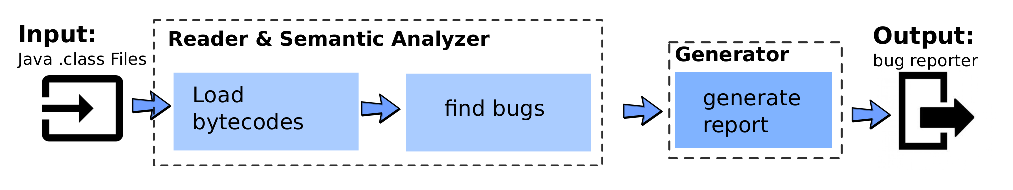
\includegraphics[scale=0.9]{Imagens/pipelineFindbugs}
	\label{fig:findBugs}
	\caption{Fase do pipiline do FindBugs.}
\end{figure}


Especificamente no caso deste trabalho, percebeu-se a necessidade de construç\~{a}o de um software que 
realiza a an\'{a}lise est\'{a}tica de c\'{o}digo para identificar tanto o uso quanto as oportunidades do uso de construç\~{o}es 
sint\'{a}ticas / sem\^{a}nticas da linguagem Java. Em termos arquiteturais, a Figura:~\ref{fig:stagesAnalyzer} ilustra, 
em um alto n\'{i}vel de abstra\c c\~{a}o, os principais componentes que formam o \emph{pipeline} do analisador est\'{a}tico 
implementado nesse trabalho e cujos detalhes de implementa\c c\~{a}o s\~{a}o apresentados no pr\'{o}ximo cap\'{i}tulo.

\begin{figure}[h]
	\center
	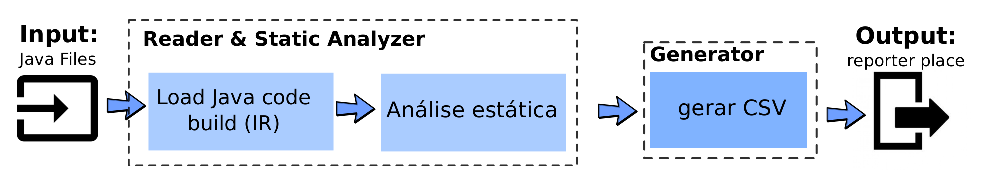
\includegraphics[scale=0.9]{Imagens/stagesAnalizer}
	\label{fig:stagesAnalyzer}
	\caption{Ferramentas necess\'{a}rias para construç\~{a}o do analisador est\'{a}tico.}
\end{figure}

O analisador desenvolvido neste trabalho \'{e} considerado um {\it grammarware} pois \'{e} um software que depende da gram\'{a}tica da linguagem Java para seu funcionamento pois tais softwares devem possum s\'{o}lido conhecimento da  gram\'{a}tica que manipulam. Como exemplos de arquiteturas que possuem tal conhecimento tem-se os programas de convers\~{a}o de dados, processadores de \texttt{XML} e os softwares que efetuam \textit{parses}.

Paul Klint at.al.~\cite{klint2005toward} vai mais al\'{e}m para caracterizar um {\it grammarware} como sendo um software comum, afirmando que este deve  adotar t\'{e}cnicas contempor\^{a}neas a engenharia de software tendo em vista que tais t\'{e}cnicas s\~{a}o utilizadas diariamente no desenvolvimento n\~{a}o sendo nenhuma novidade. A contemporaneidade deste analisador da-se por utilizar t\'{e}cnicas para inje\c{c}\~{a}o de depend\^{e}ncia, controle de dep\^{e}ndencia e  reposit\'{o}rio para manter gerenciamento do software.

Gram\'{a}ticas e software dependentes de gram\'{a}tica n\~{a}o s\~{a}o inven\c{c}\~{o}es recentes e este conceito faz-se presente em \'{a}reas da computa\c{c}\~{a}o como engenharia reversa, desnvolvimento orientado a aspectos, tranforma\c{c}\~{o}es de programas e metamodelagem.

Alguns cen\'{a}rios favorecem o desenvolvimento de softwares {\it grammarware}, onde dentre os diversos cen\'{a}rios pode-se destacar uma aplicaç\~{a}o que necessite importar perfis de usu\'{a}rios para promover a transi\c{c}\~{a}o da vers\~{a}o antiga para uma vers\~{a}o atual. Esta transi\c{c}\~{a}o deve ser robusta e provavelmente necessitar\'{a} de adpta\c{c}\~{a}o o que em muitos casos necessita de um \textit{parser} para partes que necessitam ser adaptadas.

Um outro cen\'{a}rio real \'{e} desenvolvimento de aplica\c{c}\~{o}es de banco de dados onde \'{e} necess\'{a}rio adotar uma nova linguagem de defini\c{c}\~{a}o para um ambiente espec\'{i}fico. De forma que automatizar esta solu\c{c}\~{a}o requer o uso de um \textit{parser} o qual ser\'{a} respons\'{a}vel por identificar os inputs de entrada para efetuar o mapeamento correto para a sa\'{i}da desejada no formato mais atual.

Outro tipo de \textit{software} que manipula a gram\'{a}tica de uma linguagem,s\~{a}o os que realizam \textit{refactoring}. Dentre diversas caracter\'{i}sitas explicadas por Martin Fowler at.al.~\cite{martinFowlerRafactoring}, fica claro que este trabalho contribui com o intu\'{\i}to de identificar constru\c{c}\~{o}es obsoletas e oportunidades para alguma evolu\c{c}\~{a}o e n\~{a}o efetuando \textit{refactoring} de modo autom\'{a}tico mas sim sugerindo ao desenvolvedor escolher pela evolu\c{c}\~{a}o ou n\~{a}o.

A evolu\c{c}\~{a}o do c\'{o}digo para um mais atual \'{e} mais que procurar por \textit{bad smell} onde s\~{a}o ocorr\^{e}ncias pontuais j\'{a} estabelecidas. A oportunidade de evoluir para uma vers\~{a}o mais atual \'{e} muito mais complexa que meramente melhorar o desgin do \textit{software} e por isso essa sugest\~{a}o deve ser apreciada pelo desenvolvedor com cuidado pois pode ser um quest\~{a}o mais profunda. %depender de SO, versao de compilador etc.

Mesmo sem a implementa\c{c}\~{a}o de \textit{refactoring} uma contribui\c{c}\~{a}o que este trabalho faz \'{e} a identifi\c{c}\~{a}o a capacidade de encontrar c\'{o}digo duplicado como por exemplo ao identificar \texttt{catch} repetidos, ou at\'{e} mesmo melhorar o desempenho com no caso da da utilizaç\~{a}o do \texttt{switch-string} ao inv\'{e}s do \texttt{if-string} pois oracle afirma que o desempenho \'{e} melhor de a implementa\c{c}\~{a}o otimizada do \texttt{switch-string} na documenta\c{c}\~{a}o~\cite{docSwitch}.




%Pode-se compreender este analisador como um \emph{grammarware}~\cite{} pois \'{e} um software 
%que depende fortemente de uma gram\'{a}tica para seu funcionamento--- neste caso a gram\'{a}tica da linguagem Java. 
%%\emph{Grammawares} demandam um conhecimento essencial das  gram\'{a}ticas que manipulam. 
%%Como exemplos de arquiteturas que possuem tal conhecimento tem-se os programas de convers\~{a}o de dados, processadores de \texttt{XML} e os que efetuam \textit{parses}.
%De acordo com~\cite{}, alguns cen\'{a}rios favorecem o desenvolvimento de softwares alinhados com a abordagem 
%\emph{grammarware}, com destaque \`{a}s aplicaç\~{o}es que necessitam importar perfis de usu\'{a}rios para promover a transiç\~{a}o da vers\~{a}o 
%antiga para uma vers\~{a}o nova {\color{red}[rba] n\~{a}o consegui entender bem essa senten\c ca}. 
%Esta transiç\~{a}o deve ser robusta e provavelmente necessitar\'{a} de adptaç\~{a}o dever\'{a} passar 
%por um parser para que as partes que necessitem de adaptaç\~{a}o possam ser identificadas.
%
%Um outro cen\'{a}rio real \'{e} o desenvolvimento de aplicaç\~{o}es de banco de dados onde se faz necess\'{a}rio adotar 
%uma nova linguagem de definiç\~{a}o para um ambiente espec\'{i}fico. De forma que automatizar esta soluç\~{a}o requer o uso de um 
%parser que ser\'{a} respons\'{a}vel por reconhecer as entradas necess\'{a}rias para efetuar o mapeamento 
%para a \emph{linguagem} destino.


%% Um \textit{software} que efeta manipula\c{c}\~{a}o da gram\'{a}tica de uma linguagem, como no caso deste trabalho de conclus\~{a}o fica evidente o aparecimento da quest\~{a}o sobre \textit{refactoring} e dentre diversas caracter\'{i}sitas explicadas por Martin Fowler~\cite{martinFowlerRafactoring}, fica claro que este trabalho contribui com o intu\'{\i}to de identificar constru\c{c}\~{o}es obsoletas n\~{a}o efetuando \textit{refactoring} autom\'{a}tico mas fazendo  com que o desenvolvedor opte pela evolu\c{c}\~{a}o ou n\~{a}o. Pois a evolu\c{c}\~{a}o do c\'{o}digo por um mais atual \'{e} uma das oportunidades de melhorar o desgin do \textit{software} conforme aborda por Martin Fowler~\cite{martinFowlerRafactoring} em seu livro.

%% Mesmo sem a implementa\c{c}\~{a}o de \textit{refactoring} uma contribui\c{c}\~{a}o que este trabalho faz \'{e} a identifi\c{c}\~{a}o a capacidade de encontrar c\'{o}digo duplicado como por exemplo ao identificar \texttt{catch} repetidos, ou at\'{e} mesmo melhorar o desempenho com no caso da da utilizaç\~{a}o do \texttt{switch-string} ao inv\'{e}s do \texttt{if-string} pois oracle afirma que o desempenho \'{e} melhor de a implementa\c{c}\~{a}o otimizada do \texttt{switch-string} na documenta\c{c}\~{a}o~\cite{docSwitch}.




%Atualmente a evoluç\~{a}o de uma linguagem de programaç\~{a}o ocorre predominantemente de forma {\it ad-hoc} e em muitos casos manualmente, para a traduç\~{a}o de aplicativos legados, conforme a demanda. A ferramentas de an\'{a}lise para gerar a evoluç\~{a}o necess\'{a}ria, {\it grammarware}, tende a condizir este processo abordando a classe gramatical que deve ser evolu\'{i}da. Neste caso analisador que muitas vezes realizaria o trabalho por tentativa e erro, tem como base a gram\'{a}tica do c\'{o}digo a ser analisado. Especificaç\~{o}es do analisador s\~{a}o derivados automaticamente da semi gram\'{a}tica. Diferentes tecnologias de an\'{a}lise que podem ser orientadas em oposiç\~{a}o a uma tecnologia espec\'{i}fica. Assim o processo de personalizaç\~{a}o/evoluç\~{a}o \'{e} suscept\'{i}vel de exigir a entrada de um engenheiro de {\it grammarware} o qual tem conhecimento pr\'{e}vio da gram\'{a}tica a ser analisada.

%Um ponto cr\'{i}tico quanto a an\'{a}lise de c\'{o}digo fonte \'{e} o \textit{parser} da linguagem, onde \'{e} necess\'{a}rio reconhecer uma frase para efetuar a interpretaç\~{a}o ou fazer a traduç\~{a}o para que a criaç\~{a}o da representaç\~{a}o intermedi\'{a}ria aconteça. Inicialmente \'{e} necess\'{a}rio identificar se a frase que ser\'{a} tratada \'{e} um \textit{assignment} ou uma chamada de funç\~{a}o.
 
%Reconhecer uma frase acarreta em duas coisas, distingui-la de outras construç\~{o}es e identificar os elementos e as subestruturas que comp\~{o}em esta frase. Por exemplo se uma frase for reconhecida como um \textit{assignment}, pode-se identificar as vari\'{a}veis a esquerda do operador \texttt{=} e uma express\~{a}o que \'{e} a subestrutura a direita. Este ato de reconhecer uma frase \'{e} denominado \textit{Parse}.


%\section{Parse}

%Confome discutido anteriormente, o parser de programas escritos em uma linguagem de program\c c\~{a}o 
%\'{e} um dos componentes necess\'{a}rios para a constru\c c\~{a}o de ferramentas de an\'{a}lise 
%est\'{a}tica. Vale ressaltar que o analisador est\'{a}tico constru\'{i}do neste trabalho reusou uma infraestrutura 
%da plataforma Eclipse~\cite{} que oferece um parser atualizado da linguagem Java. Por outro lado, como 
%se trata de um tipo de componente central para solu\c c\~{o}es baseadas em gram\'{a}tica, esta se\c c\~{a}o 
%revisa brevemente quatro padr\~{o}es adotados para a implementa\c c\~{a}o de parsers~\cite{Parr:2009:LIP:1823613}. S\~{a}o eles: 
%
%{\color{red}Por favor, revisem essa se\c c\~{a}o.}

\section{Representa\c{c}\~{a}o Intermedi\'{a}ria {\color{red}Se\c{c}\~{a}o Revisada -Parser-.}}\label{sec:IR}

Conforme introduzido anteriormente na Figura:~\ref{fig:stagesAnalyzer}, \'{e} gerar uma representa\c{c}\~{a}o intermedi\'{a}ria da linguagem Java. Para efetuar essa tarefa é necessário antes de tudo reconhecer \texttt{frases} entretanto para criar um reconhecimento de \texttt{frases} faz-se necessário duas etapas. Distinguir as contruções que compoem a linguagem e identificar os elementos e subestruturas das \texttt{frases}. Terrance Parr em ~\cite{Parr:2009:LIP:1823613}, explica que o ato de reconhecer \texttt{frase} em computa\c{c}\~{a}o é denominado \textit{parser}.

A estrutura do \textit{parser} \'{e} composta de maneira similar as senten\c{c}as da l\'{\i}ngua portuguesa, identificando verbos, nomes, substantivos, etc... De modo similar \'{e} necess\'{a}rio fazer a mesma identifica\c{c}\~{a}o em um linguagem de programa\c{c}\~{a}o, reconhecendo operadores, vari\'{a}veis e outros s\'{\i}mbolos. E a combina\c{c}\~{a}o dos s\'{i}mbolos \'{e} denominado \texttt{tokens}.

A representa\c{c}\~{a}o do \textit{parser} \'{e} feita atrav\'{e}s de uma árvore onde Tokens ficam nas folhas e estas  compoem as frases. \'{E} utilizando uma \'{a}rvore para representar porque com esta \'{e} poss\'{\i}vel extair toda informa\c{c}\~{a}o que seja necess\'{a}ria da linguagem. A Figura:~\ref{fig:treeParse} exibe com mais detalhes o parser sendo representado por uma \'{a}rvore.

\begin{figure}[h]
	\center
	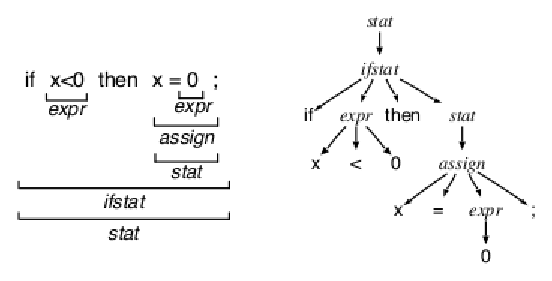
\includegraphics[scale=0.9]{Imagens/treeParser}
	\label{fig:treeParse}
	\caption{Representa\c{c}\~{a}o da uma frase.}
\end{figure}


Existem muitos padr\~{o}es de parses pois algumas linguagens s\~{a}o mais complexas que outras. Tendo em visata o desafio que \'{e} trabalhar e analisar uma linguagem de programa\c{c}\~{a}o, alguns padr\~{o}es adotados para este contexto facilitam esta tarefa e com isso este trabalho abordar\'{a} os quatro conceitos  mais importantes segundo Terence Parr em \cite{Parr:2009:LIP:1823613} para prover o parser de acordo com a necessidade.
\begin{itemize}
	\item \textbf{Mapping Grammars to Recursive-Descent Recognizers}\\
	Sua proposta \'{e} traduzir uma gram\'{a}tica para uma recurs\~{a}o descendente para reconhecer frases e sentenças em uma linguagem especificada por uma gram\'{a}tica. Este padr\~{a}o identifica o n\'{u}cleo do fluxo de controle para qualquer recurs\~{a}o descendente e \'{e} utilizado nos 3 padr\~{o}es seguintes. 
	Para construir um reconhecedor l\'{e}xico ou \textit{parsers} manualmente o melhor ponto de in\'{i}cio \'{e} a gram\'{a}tica, com isso este padr\~{a}o fornece uma maneira simples de construir reconhecedores diretamente de sua gram\'{a}tica.
	
	\item \textbf{LL(1) Recursive-Descent Lexer}\\
	O objetivo deste padr\~{a}o \'{e} para emitir uma sequência de s\'{i}mbolos. Cada s\'{i}mbolo tem dois atributos prim\'{a}rios: um tipo de \textit{token}(s\'{i}mbolo da categoria) e o texto associado por exemplo 
	no português, temos categorias como verbos e substantivos, bem como s\'{i}mbolos de pontuaç\~{a}o, como v\'{i}rgulas e pontos. Todas as palavras dentro de uma determinada categoria s\~{a}o do mesmo tipo de \textit{token}, embora o texto associado seja diferente. O tipo de nome do \textit{token} representa o categoria identificador. Ent\~{a}o precisamos tipos de \textit{token} para o vocabul\'{a}rio \textit{string} fixa s\'{i}mbolos como tamb\'{e}m lidar com espaços em branco e coment\'{a}rios.
	\item \textbf{LL(1) Recursive-Descent Parser}\\
	Esse \'{e} o mais conhecido padr\~{a}o de an\'{a}lise descendente recursiva. Ele s\'{o} precisa	a olhar para o s\'{i}mbolo de entrada atual para tomar decis\~{o}es de an\'{a}lise. Para cada regra de gram\'{a}tica, existe um m\'{e}todo de an\'{a}lise no analisador. Este padr\~{a}o analisa a estrutura sint\'{a}tica da sequência sinal de uma frase usando um \'{u}nico \textit{token} \textit{lookahead}. Este analisador pertence à LL(1) classe do analisador de cima para baixo, em especial, porque usa um \'{u}nico sinal de verificaç\~{a}o à frente (da\'{i} o "1" no nome). É o principal mecanismo de todos os padr\~{o}es de an\'{a}lise subsequentes. Este padr\~{a}o mostra como implementar as decis\~{o}es de an\'{a}lise que utilizam um s\'{i}mbolo \'{u}nico da vis\~{a}o antecipada. É a forma mais fraca de descendente recursivo parser, mas o mais f\'{a}cil de compreender e aplicar.
	\item \textbf{LL(k) Recursive-Descent Parser}\\
	Este padr\~{a}o utiliza a o modo \textit{top-down} para percorrer um \'{a}rvore sem\^{a}ntica com o aux\'{i}lio de express\~{o}es booleanas que ajudam na tomada de decis\~{a}o e estas express\~{o}es s\~{a}o conhecidas como predicados sem\^{a}nticos.
\end{itemize}


O principal motivo da representa\c{c}\~{a}o intermedi\'{a}ria ser uma \'{a}rvore \'{e} por possuir uma estrutura regular e com os n\'{o}s preservam a hierarquia, devido essa regularidade \'{e} poss\'{i}vel automatizar esta tarefa utilizando ferramentas como no caso deste trabalho a biblioteca Eclipse JDT a qual possui classes especializadas em gerar e analisar as representa\c{c}\~{o}es intermedi\'{a}rias dos c\'{o}digo fonte da linguagem Java.




\section{Refactoring}\label{sec:refactoring}

Por defini\c{c}\~{a}o o refactoring \'{e} mudan\c{c}a interna do software sem alterar seu comportamento tornando assim seu entendimento mais claro. Visando evitar que sejam perdidas diversa horas para identificar poss\'{\i}veis oportunidades de classes onde possam ser evolu\'{\i}das, este trabalho de conclus\~{a}o identifica trechos de c\'{o}digo dentro das classes que pode ser evolu\'{i}dos.

Muitas modifica\c{c}\~{o}es podem ser feitas em um software mas segundo M.Fowler at al~\cite{martinFowlerRafactoring} somente \'{e} considerado refactoring mudan\c{c}as que facilitam o entendimento do software. Contrastando esta vis\~{a}o existem mudanças com objetivo de melhorar o desempenho do software onde somente s\~{a}o alterada as estruturas internas permanecendo inalterado o comportamento do software. Entretanto a melhoria na performance do software geralmente eleva o grau de dificuldade para sua compreens\~{a}o, o que faz com que algumas dessas evolu\c{c}es\~{o} visando desempenho n\~{a}o sejam caracterizadas como refactoring dado a defini\c{c}\~{a}o.

Dentre refatorar para facilitar o entendimento, para tornar o programa mais r\'{a}pido, para encontrar bugs e para melhorar/atualizar o design, motivos apresentados por M.Fowler at. al.~\cite{martinFowlerRafactoring}, este trabalho concentrou-se no \'{u}ltimo motivo para identificar poss\'{\i}veis casos onde o design do software pode ser evolu\'{\i}do por substituir funcionalidades de vers\~{o}es anteriores da linguagem Java.

Um software que n\~{a}o \'{e} refatorado tem o seu desgin deteriorado, o que leva a dificultar o entendimento do c\'{o}digo. Um design ultrapassado tem mais c\'{o}digo que o necess\'{a}rio para realizar a mesma tarefa. O que leva a um aspecto crucial para a melhoria, que \'{e} código duplicado. Vale ressaltar que reduzir a quantidade de c\'{o}digo n\'{a}o impl\'{i}ca necessariamente na melhora do desempenho do software mas sim em ter um design mais atual.

O Listing:~\ref{lst:fp}, exemplifica de forma emp\'{i}rica um {\it filter} em um {\it collection} onde ocorre uma redu\c{c}\~{a}o significativa de c\'{o}digo al\'{e}m de um design mais atual por utilizar express\~{o}es lambda que foram adicionadas em Java 8. Vale destacandar que o Listing:~\ref{lst:fp} continua com mesmo comportamento após o refactoring, desta forma nenhum usuário ou desenvolvedor pode alegar que o software foi modificado.


\begin{lstlisting}[caption={The \textsc{Exmplo de Filter Pattern}}\label{lst:fp},language=Java] 
//...
for(T e: collection) {
   if(e.pred(args)) {
      otherCollection.add(e);
   }
}

//might be replaced by:
collection.stream().
	filter(e->pred(args).
		forEach(e -> otherCollection.add(e));
\end{lstlisting}


Conforme explica M.Fowler at. al.~\cite{martinFowlerRafactoring} algumas vezes n\~{a}o se deve ser refatorar o c\'{o}digo. Um desses casos \'{e} quando existir a necessidade de reescrever todo o c\'{o}digo, um outro caso \'{e} a necessidade de manter um  c\'{o}digo de f\'{a}cil entendimento para os programadores iniciantes. O que \'{e} uma decis\~{a}o dif\'{i}cil, no caso do Listing:~\ref{lst:fp} \'{e} poss\'{\i}vel fazer uma evolu\c{c}\~{a}o com a parte funcional de Java 8 entretanto alguns desenvolvedores podem n\~{a}o possuir  conhecimento adequado da parte funcional e com isso \'{e} recomendado que n\~{a}o seja evolu\'{\i}do o c\'{o}digo.


Tendo em vista que aplicar um \textit{refactoring} demanda tempo isto torna uma tarefa custosa para empresas, este fator \'{e} determinante para que programadores n\~{a}o refatorem seu c\'{o}digos em muitos casos. Com esse cen\'{a}rio \'{e} imprecind\'{i}vel o uso de ferramentas refatorem ou auxiliem nesta tarefa. Auxiliando nesta tarefa este trabalho identifica possibilidades de refatora\c{c}\~{a}o, ao utilizarem estas ferramentas torna mais acessível ao programador e a emrpesa refatorar pois o trabalho é direcionado fazendo com que tempo seja poupado.



\section{Análise estática}\label{sec:as}

Em computa\c{c}\~{a}o an\'{a}lise est\'{a}tica \'{e} a refer\^{e}ncia a qualquer processamento realizado em c\'{o}digo fonte sem a necessidade de execut\'{a}-lo, com isto a an\'{a}lise est\'{a}tica torna-se uma poderosa t\'{e}cnica por permitir r\'{a}pidas considera\c{c}\~{o}es por possibilitar uma larga explora\c{c}\~{a}o em um projeto podendo evitar erros triviais e simular alguns cen\~{a}rios para tal an\'{a}lise sem a necessidade do projeto ser executado.

Ferramentas que auxiliem a an\'{a}lise est\'{a}tica tem grande chance de ser um poderoso aux\'{i}lio no desenvolvimento do software tendo em vista que pode reduzir a quantidade de erros e diminuir a quantidade de \texttt{refactoring} o qual tem um custo elevado para os projetos de software.

\'{E} nesse contexto que este trabalho faz sua contribui\c{c}\~{a}o por utilizar a an\'{a}lise est\'{a}tica para verificar n\~{a}o possibilidade de falhas ou \textit{bad smell}, mas sim de identificar chances reais de evoluir para \'{u}ltimas \textit{features} da linguagem Java sem interferir no comportamento interno do programa conforme preconiza M.Fowler at. al.~\cite{martinFowlerRafactoring}.

A linguagem Java proporciana duas maneiras de realizar an\'{a}lise est\'{a}tica, a primeira \'{e} através c\'{o}digo fonte, \textit{.java} e a segunda atrav\'{e}s do \textit{bytecode}, \textit{.class}. Este trabalho foca em realizar an\'{a}lise no c\'{o}digo fonte, entre tanto nada impede que o trabalho seja realizado da segunda maneira. Existem programas renomados que realizam tal an\'{a}lise utilizando os \textit{bytecodes} e um destes programas \'{e} o FindBugs~\cite{FindBugs}.

%Análise estática é uma técnica automática no processo de verificação de software realizado por algumas ferramentas sem a necessidade de que o software tenha sido executado. Para Java exitem duas possibilidades de realizar tal análise na qual uma das técnicas realiza a primeira \'{e} aanálise no código fonte e a outra a realiza no {\it bytecode} do programa segundo N. Ayewah at. al. ~\cite{Ayewah:2008:USA:1439186.1439221}. Neste trabalho ser utilizada a pesquisa baseada no código fonte sem que tenha sido executado devido a flexibilidade e infraestrutura consolidada encontrada no Eclipse AST.

Para obter sucesso atrav\'{e}s nas an\'{a}lises realizadas, \'{e} necess\'{a}rio determinar padr\~{o}es para encontrar caracter\'{i}sticas que dejesam ser evolu\'{i}das para a \'{u}ltima vers\~{a}o da linguagem Java. Estes padr\~{o}es s\~{a}o estabelecidos em uma estrutura que seja capaz de pesquisar nos n\'{o}s da \'{a}rvore da representa\c{c}\~{a}o intermedi\'{a}ria para extrair as informa\c{c}\~{o}es pertinentes.

%Um fato importante é que tal análise somente obt\'{e}m sucesso se forem determinados padr\~{o}es ou comportamento para que sejam pesquisados no software. Neste projeto o tais comportamentos são determinados por {\it visitors} conforme explica Gamma et. al. ~\cite{Gamma:1995} devido a toda infraestrutura a qual as ferramentas do eclipse fornecem facilidade para que seja realizada uma análise baseada em padrões.

A t\'{e}cnica utilizada para pesquisar nos n\'{o}s das \'{a}rvores foi utilizar o padr\~{a}o de projeto \textit{Visitor} proposto por  Gamma et. al.~\cite{Gamma:1995}, pois este possibilitar que seja realizada uma opera\c{c}\~{a}o sobre todos os elementos de uma estrutura,  neste caso a opera\c{c}\~{a}o  \'{e} a pesquisa e a estrutura a representa\c{c}\~{a}o intermedi\'{a}ria.


A verifica\c{c}\~{a}o de software possibilita a detec\c{c}\~{a}o de falhas de maneira precoce durante as fases de desenvolvimento entretanto este n\~{a}o \'{e} o objetivo deste trabalho pois existem ferramentas consolidadas que realizam tal an\'{a}lise de maneira excepcional. Aqui o objetivo principal \'{e} alertar ao desenvolvedor a possibilidade de usar o que h\'{a} de mais recente na linguagem Java.

%Devido a este trabalho de verificação de software é possível detectar falhas de forma precoce nas fases de  desenvolvimento evitando que bugs e falhas sejam introduzidas e até mesmo postergados e isso é uma vantagem existe a economia de tempo com falhas simples, {\it  feedback} rápido para alertar a equipe devido as falhas ocorridas e pode-se ir além de simples casos de testes podendo aprimorar estes para que  fiquem mais rigorosos pois a partir do momento que o analisador encontrar uma falha é possível criar um teste de caso para que esta seja testada aumentando a confiabilidade do software.

%Existe limita\c{c}\~{a}o quanto a capacidade dos analisadores est\'{a}ticos como em \textit{software} desenvolvidos sem qualquer uso de padrões ou sem arquiteturas consolidadas, criado por equipes composta de desenvolvedores inexperientes o qual a ferramente poderá apontar erros que são falsos positivos que são erros detectados que não existem pois o analisador pesquisa por padrões e estruturas consolidadas. Tais problemas são desagradáveis porém não oferecem riscos ao desenvolvimento, podem afetar outras áreas como a de {\it refactoring} a qual poderá encontrar dificuldade em melhorar um código que não segue padrão. Vale ainda ressaltar que a penalidade de encontrar um falso positivo é a perda de tempo em fazer uma inspeção no código para comprovar se é ou não uma falha. Também há a possibilidade de falsos negativos o que cabe ao programador verificar para evitar que tais limitação do analisador não se propague durante o ciclo de desenvolvimento.


%A capacidade dos analisadores est\'{a}ticos 


%	\section {Análise léxica}
	Ferramentas que operam em código-fonte conforme \cite{Wichmann95industrialperspective} começam por transformar o código em um série de {\it tokens}, descartando recursos sem importância de o texto do programa, tais como espaços em branco ou comentários ao longo do caminho. A criação do fluxo de sinal é chamado de análise lexical. Regras léxicas muitas vezes usam expressões regulares para identificar fichas.
	Observa-se que a maioria dos {\it tokens} são representados inteiramente por seu tipo, mas para ser útil, o {\it tokens} de identificação requer uma peça adicional de informação: o nome do identificador. Para habilitar o relatório de erro útil mais tarde, os {\it tokens} devem transportar pelo menos um outro tipo de informação com eles: a sua posição no texto-fonte (geralmente um número de linha e um número de coluna). Para as mais simples ferramentas de análise estática, o trabalho está quase concluído neste ponto. Se toda a ferramenta tem que fazer é combinar os nomes de funções, o analisador pode ir através do fluxo de {\it tokens} procurando identificadores, combiná-los com uma lista de nomes de funções, e relatar o resultados.
	
	\section{Parser}
	Um analisador de linguagem usa uma gramática livre de contexto (CFG) indicado por \cite{Chess:2007:SPS:1406221} para coincidir com os {\it tokens} correntes. A gramática é composta por um conjunto de produções que descrevem os símbolos (elementos) na língua. No Exemplo é enumerado um conjunto de produções que são capazes de analisar o fluxo de {\it tokens} de amostra.
	
	\begin{lstlisting}
	stmt := if_stmt | assign_stmt
	if_stmt := IF LPAREN expr RPAREN stmt
	expr := lval
	assign_stmt := lval EQUAL expr SEMI
	lval = ID | arr_access
	arr_access := ID arr_index+
	arr_idx := LBRACKET expr RBRACKET
	\end{lstlisting}
	
	O analisador executa uma derivação, combinando o fluxo de sinal contra as regras de produção. Se cada símbolo é ligado a partir da qual o símbolo foi derivado, uma árvore de análise é formada. Na Figura: \ref{fig:TreeParser} mostra uma árvore de análise criada, usando as regras de produção do exemplo anterior. Omiti-se terminais de símbolos que não carregam nomes \textit{(IF, LPAREN, RPAREN, etc.}), para fazer o principais características da árvore de análise mais óbvia.
	
	\begin{figure}[h]
		\center
		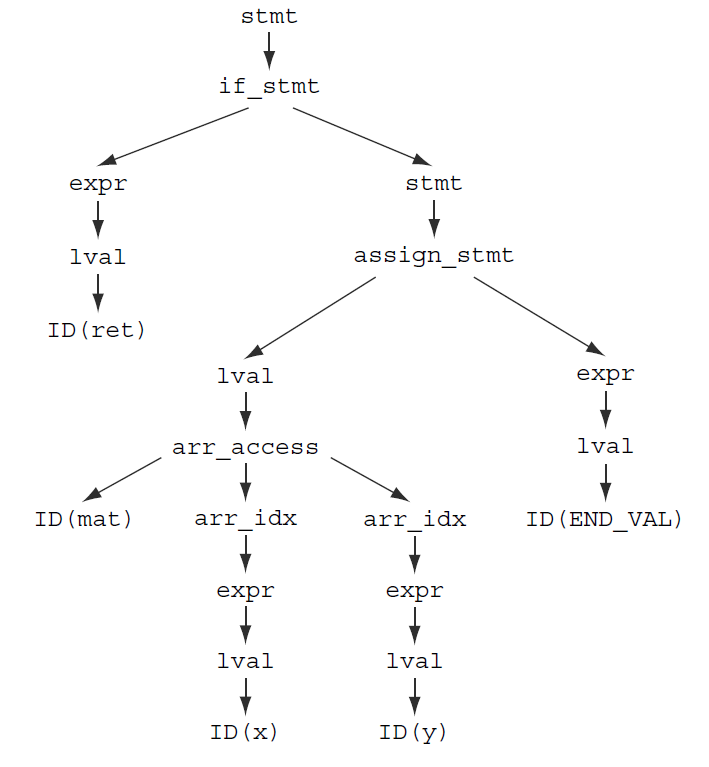
\includegraphics[width=0.8\textwidth]{Imagens/Arvore}
		\label{fig:TreeParser}
		\caption{Árvore de parser.}
	\end{figure}
	
	
	\subsection{Paser JDT Eclipse}
	No caso do \textit{parser} provido pela infraestrutura \textit{JDT} do eclipse,  a classe \textit{ASTParser} contida na biblioteca \textit{org.eclipse.jdt.core.dom} permite a criação de uma árvore de sintaxe abstrata.\\
	Este procedimento é realizado em todos os aquivos \textit{.java} contido em um projeto e com isso cada um possui uma referência de \textit{CompilationUnit} o qual permite acesso ao nó raiz árvore sintática de cada arquivo. O parse é gerado conforme as últimas definições da linguagem utilizando \textit{AST.JLS8}.\

	\begin{lstlisting}
		ASTParser parser = ASTParser.newParser(AST.JLS8);
		
		Map<String, String> options = JavaCore.getOptions();
		options.put(JavaCore.COMPILER_COMPLIANCE, JavaCore.VERSION_1_8);
		options.put(JavaCore.COMPILER_CODEGEN_TARGET_PLATFORM, JavaCore.VERSION_1_8);
		options.put(JavaCore.COMPILER_SOURCE, JavaCore.VERSION_1_8);
		
		parser.setKind(ASTParser.K_COMPILATION_UNIT);
		parser.setCompilerOptions(options);
		parser.setSource(contents);
		
		final CompilationUnit cu = (CompilationUnit) parser.createAST(null);
		return cu;
	\end{lstlisting}
	
	Neste, o \textit{parser} é realizado através de uma classe denominada de mesmo nome, a qual é instanciada um única vez no projeto através do padrão \textit{singleton} \cite{Gamma:1995}.
	

	\section{Sintaxe abstrata}
	É possível fazer uma análise significativa em uma árvore de parser, e certos tipos de checagem estilísticas são mais bem executadas em uma árvore de análise, pois contém mais representações diretas do código assim como o programador escreve. No entanto, executar análise complexa em uma árvore de análise pode ser inconveniente. Os nós da árvore são derivados diretamente das regras de produção da gramática, e essas regras podem-se introduzir símbolos não terminais que existem apenas para fins de fazer a análise mais fácil e menos ambígua, ao invés de para o objetivo de produzir uma facilmente compreendido a árvore. É geralmente melhor para abstrair ambos os detalhes da gramática e as estruturas sintáticas presente no código fonte do programa. Uma estrutura de dados que faz estas coisas é chamado de uma árvore de sintaxe abstrata (AST). O objectivo da AST é fornecer uma versão padronizada do programa adequado para posteriores análises. A AST é normalmente construída associando código construção árvore com regras de produção da gramática. A Figura: \ref{fig:ArvoreAST} mostra uma AST. Observa-se que a instrução {\it if} agora tem uma outra ramificação vazia, o predicado testado pelo caso é agora uma comparação explícita para zero (o comportamento exigido pelo C), e acesso à matriz é uniformemente representada como uma operação de binário.
	
	\begin{figure}[h]
		\center
		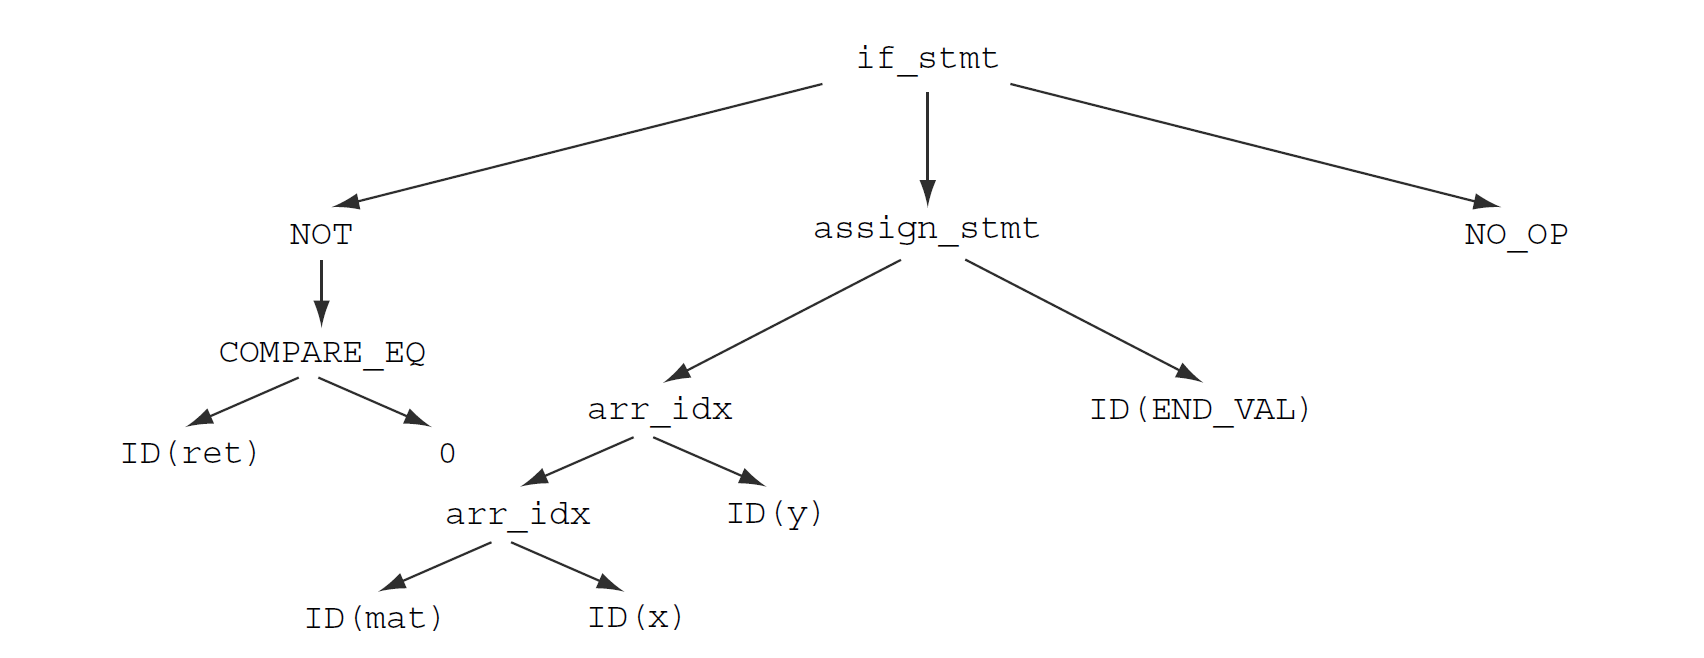
\includegraphics[width=1\textwidth]{Imagens/ArvoreAST}
		\label{fig:ArvoreAST}
		\caption{Árvore AST.}
	\end{figure}

	\section{Análise semântica}
	Como a AST está sendo construída, a ferramenta cria uma tabela de símbolos ao lado dela. Para cada identificador no programa, a tabela de símbolos associa o identificador com seu devido tipo e um ponteiro para a sua declaração ou definição. Com a AST e a tabela de símbolo, a ferramenta está agora equipado-se para realizar a verificação de tipo. A ferramenta de análise estática não pode ser obrigados a comunicar erros de checagem de tipo da maneira um compilador faz, mas informações de tipo é criticamente importante para a análise de uma linguagem orientada a objetos, porque o tipo de um objeto determina o conjunto de métodos que o objeto pode invocar. Além disso, é normalmente desejável para converter, pelo menos, as conversões do tipo implícito no código fonte para conversões de tipo explícitas no AST. Por estas razões, uma ferramenta de análise estática avançado tem a ver apenas como muito trabalho relacionado com a verificação de tipo como um compilador faz. No mundo do compilador, resolução de símbolo e verificação de tipo são referidos como análise semântica porque o compilador está atribuindo significado aos símbolos encontrada no programa. As ferramentas de análise estática que usam essas estruturas de dados têm uma vantagem distinta sobre ferramentas que não o fazem. Por exemplo, eles podem interpretar corretamente o significado dos operadores sobrecarregados em C++ ou determinar que um método em Java chamado doPost () é, na verdade, uma parte de uma implementação de HttpServlet.Estas capacidades permitem uma ferramenta para executar verificações úteis na estrutura deo programa. Após análise semântica, compiladores e a análise estática mais avançada ferramentas de formas de peça. Um compilador moderno usa a AST e o símbolo e o tipo informações para gerar uma representação intermediaria, uma versão genérico do código de máquina que é adequado para otimização e, em seguida, a conversão em específico da plataforma de código-objeto. O caminho para ferramentas de análise estática é menos clara. Dependendo do tipo de análise a ser realizada, uma ferramenta de análise estática pode executar transformações adicionais sobre a AST ou pode gerar a sua própria variedade de representação intermediária adequada às suas necessidades. Se uma ferramenta de análise estática usa sua própria representação intermediária, que, geralmente, permite a atribuição, pelo menos, ramificando, {\it looping}, e chamadas de função. A representação intermediária que uma ferramenta de análise estática usa é geralmente umvista de nível superior do programa do que a representação intermediária que um compilador usa. Por exemplo, um compilador de linguagem C, provavelmente, converter todas as referências a campos para estruturar deslocamentos em {\it byte} na estrutura pela sua representação intermediaria, enquanto uma ferramenta de análise estática mais provavelmente continuará para se referir a estrutura de campos, pelos seus nomes.%	\section {Análise léxica}
	Ferramentas que operam em código-fonte conforme \cite{Wichmann95industrialperspective} começam por transformar o código em um série de {\it tokens}, descartando recursos sem importância de o texto do programa, tais como espaços em branco ou comentários ao longo do caminho. A criação do fluxo de sinal é chamado de análise lexical. Regras léxicas muitas vezes usam expressões regulares para identificar fichas.
	Observa-se que a maioria dos {\it tokens} são representados inteiramente por seu tipo, mas para ser útil, o {\it tokens} de identificação requer uma peça adicional de informação: o nome do identificador. Para habilitar o relatório de erro útil mais tarde, os {\it tokens} devem transportar pelo menos um outro tipo de informação com eles: a sua posição no texto-fonte (geralmente um número de linha e um número de coluna). Para as mais simples ferramentas de análise estática, o trabalho está quase concluído neste ponto. Se toda a ferramenta tem que fazer é combinar os nomes de funções, o analisador pode ir através do fluxo de {\it tokens} procurando identificadores, combiná-los com uma lista de nomes de funções, e relatar o resultados.
	
	\section{Parser}
	Um analisador de linguagem usa uma gramática livre de contexto (CFG) indicado por \cite{Chess:2007:SPS:1406221} para coincidir com os {\it tokens} correntes. A gramática é composta por um conjunto de produções que descrevem os símbolos (elementos) na língua. No Exemplo é enumerado um conjunto de produções que são capazes de analisar o fluxo de {\it tokens} de amostra.
	
	\begin{lstlisting}
	stmt := if_stmt | assign_stmt
	if_stmt := IF LPAREN expr RPAREN stmt
	expr := lval
	assign_stmt := lval EQUAL expr SEMI
	lval = ID | arr_access
	arr_access := ID arr_index+
	arr_idx := LBRACKET expr RBRACKET
	\end{lstlisting}
	
	O analisador executa uma derivação, combinando o fluxo de sinal contra as regras de produção. Se cada símbolo é ligado a partir da qual o símbolo foi derivado, uma árvore de análise é formada. Na Figura: \ref{fig:TreeParser} mostra uma árvore de análise criada, usando as regras de produção do exemplo anterior. Omiti-se terminais de símbolos que não carregam nomes \textit{(IF, LPAREN, RPAREN, etc.}), para fazer o principais características da árvore de análise mais óbvia.
	
	\begin{figure}[h]
		\center
		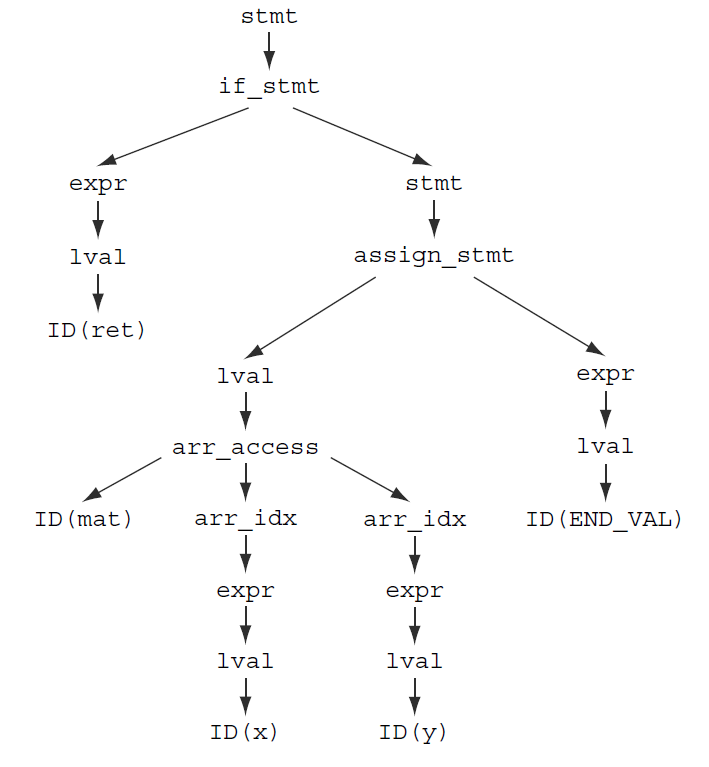
\includegraphics[width=0.8\textwidth]{Imagens/Arvore}
		\label{fig:TreeParser}
		\caption{Árvore de parser.}
	\end{figure}
	
	
	\subsection{Paser JDT Eclipse}
	No caso do \textit{parser} provido pela infraestrutura \textit{JDT} do eclipse,  a classe \textit{ASTParser} contida na biblioteca \textit{org.eclipse.jdt.core.dom} permite a criação de uma árvore de sintaxe abstrata.\\
	Este procedimento é realizado em todos os aquivos \textit{.java} contido em um projeto e com isso cada um possui uma referência de \textit{CompilationUnit} o qual permite acesso ao nó raiz árvore sintática de cada arquivo. O parse é gerado conforme as últimas definições da linguagem utilizando \textit{AST.JLS8}.\

	\begin{lstlisting}
		ASTParser parser = ASTParser.newParser(AST.JLS8);
		
		Map<String, String> options = JavaCore.getOptions();
		options.put(JavaCore.COMPILER_COMPLIANCE, JavaCore.VERSION_1_8);
		options.put(JavaCore.COMPILER_CODEGEN_TARGET_PLATFORM, JavaCore.VERSION_1_8);
		options.put(JavaCore.COMPILER_SOURCE, JavaCore.VERSION_1_8);
		
		parser.setKind(ASTParser.K_COMPILATION_UNIT);
		parser.setCompilerOptions(options);
		parser.setSource(contents);
		
		final CompilationUnit cu = (CompilationUnit) parser.createAST(null);
		return cu;
	\end{lstlisting}
	
	Neste, o \textit{parser} é realizado através de uma classe denominada de mesmo nome, a qual é instanciada um única vez no projeto através do padrão \textit{singleton} \cite{Gamma:1995}.
	

	\section{Sintaxe abstrata}
	É possível fazer uma análise significativa em uma árvore de parser, e certos tipos de checagem estilísticas são mais bem executadas em uma árvore de análise, pois contém mais representações diretas do código assim como o programador escreve. No entanto, executar análise complexa em uma árvore de análise pode ser inconveniente. Os nós da árvore são derivados diretamente das regras de produção da gramática, e essas regras podem-se introduzir símbolos não terminais que existem apenas para fins de fazer a análise mais fácil e menos ambígua, ao invés de para o objetivo de produzir uma facilmente compreendido a árvore. É geralmente melhor para abstrair ambos os detalhes da gramática e as estruturas sintáticas presente no código fonte do programa. Uma estrutura de dados que faz estas coisas é chamado de uma árvore de sintaxe abstrata (AST). O objectivo da AST é fornecer uma versão padronizada do programa adequado para posteriores análises. A AST é normalmente construída associando código construção árvore com regras de produção da gramática. A Figura: \ref{fig:ArvoreAST} mostra uma AST. Observa-se que a instrução {\it if} agora tem uma outra ramificação vazia, o predicado testado pelo caso é agora uma comparação explícita para zero (o comportamento exigido pelo C), e acesso à matriz é uniformemente representada como uma operação de binário.
	
	\begin{figure}[h]
		\center
		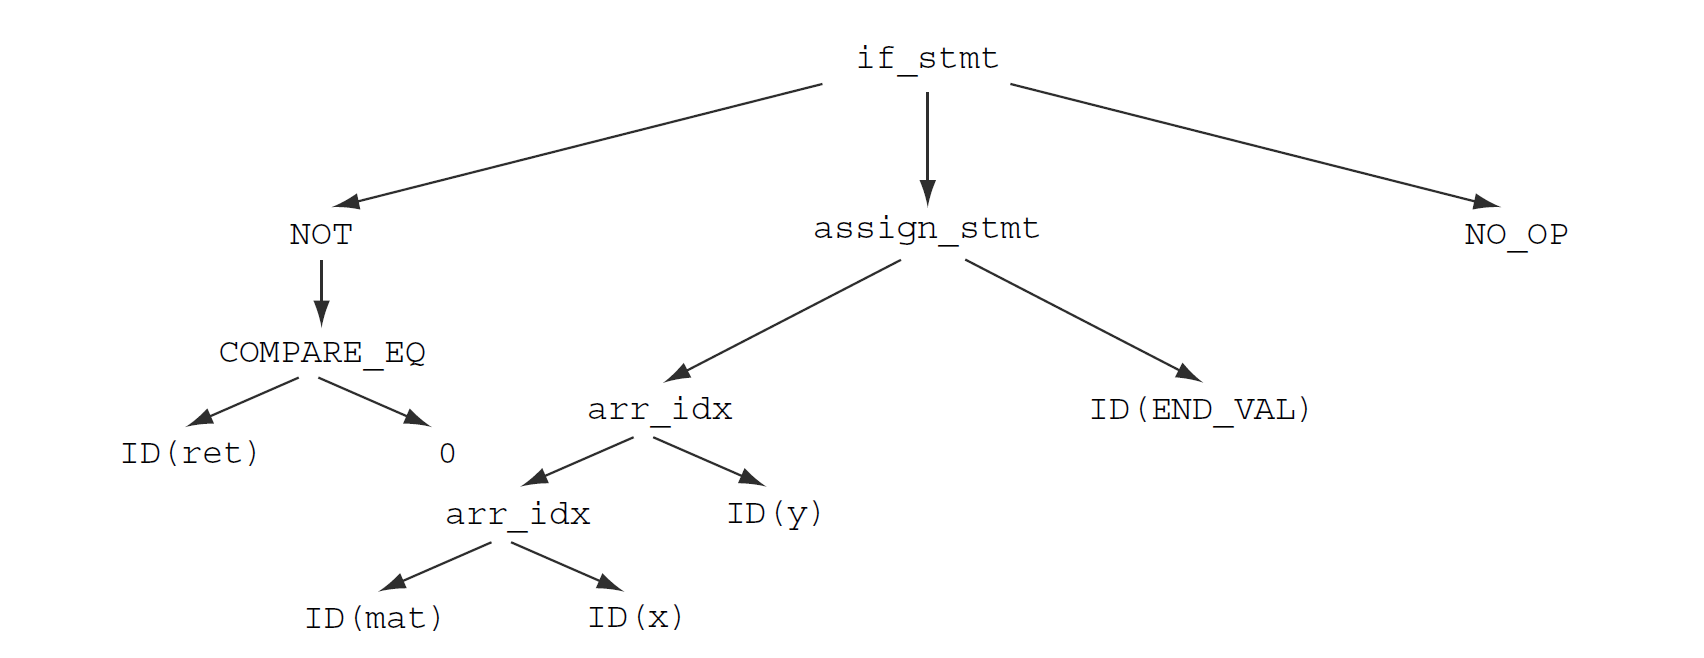
\includegraphics[width=1\textwidth]{Imagens/ArvoreAST}
		\label{fig:ArvoreAST}
		\caption{Árvore AST.}
	\end{figure}

	\section{Análise semântica}
	Como a AST está sendo construída, a ferramenta cria uma tabela de símbolos ao lado dela. Para cada identificador no programa, a tabela de símbolos associa o identificador com seu devido tipo e um ponteiro para a sua declaração ou definição. Com a AST e a tabela de símbolo, a ferramenta está agora equipado-se para realizar a verificação de tipo. A ferramenta de análise estática não pode ser obrigados a comunicar erros de checagem de tipo da maneira um compilador faz, mas informações de tipo é criticamente importante para a análise de uma linguagem orientada a objetos, porque o tipo de um objeto determina o conjunto de métodos que o objeto pode invocar. Além disso, é normalmente desejável para converter, pelo menos, as conversões do tipo implícito no código fonte para conversões de tipo explícitas no AST. Por estas razões, uma ferramenta de análise estática avançado tem a ver apenas como muito trabalho relacionado com a verificação de tipo como um compilador faz. No mundo do compilador, resolução de símbolo e verificação de tipo são referidos como análise semântica porque o compilador está atribuindo significado aos símbolos encontrada no programa. As ferramentas de análise estática que usam essas estruturas de dados têm uma vantagem distinta sobre ferramentas que não o fazem. Por exemplo, eles podem interpretar corretamente o significado dos operadores sobrecarregados em C++ ou determinar que um método em Java chamado doPost () é, na verdade, uma parte de uma implementação de HttpServlet.Estas capacidades permitem uma ferramenta para executar verificações úteis na estrutura deo programa. Após análise semântica, compiladores e a análise estática mais avançada ferramentas de formas de peça. Um compilador moderno usa a AST e o símbolo e o tipo informações para gerar uma representação intermediaria, uma versão genérico do código de máquina que é adequado para otimização e, em seguida, a conversão em específico da plataforma de código-objeto. O caminho para ferramentas de análise estática é menos clara. Dependendo do tipo de análise a ser realizada, uma ferramenta de análise estática pode executar transformações adicionais sobre a AST ou pode gerar a sua própria variedade de representação intermediária adequada às suas necessidades. Se uma ferramenta de análise estática usa sua própria representação intermediária, que, geralmente, permite a atribuição, pelo menos, ramificando, {\it looping}, e chamadas de função. A representação intermediária que uma ferramenta de análise estática usa é geralmente umvista de nível superior do programa do que a representação intermediária que um compilador usa. Por exemplo, um compilador de linguagem C, provavelmente, converter todas as referências a campos para estruturar deslocamentos em {\it byte} na estrutura pela sua representação intermediaria, enquanto uma ferramenta de análise estática mais provavelmente continuará para se referir a estrutura de campos, pelos seus nomes.